%%%%%%%%%%%%%%%%%%%%%%%%%%%%%%%%%%%%%%%%%
% baposter Portrait Poster
% LaTeX Template
% Version 1.0 (15/5/13)
%
% Created by:
% Brian Amberg (baposter@brian-amberg.de)
%
% This template has been downloaded from:
% http://www.LaTeXTemplates.com
%
% License:
% CC BY-NC-SA 3.0 (http://creativecommons.org/licenses/by-nc-sa/3.0/)
%
%%%%%%%%%%%%%%%%%%%%%%%%%%%%%%%%%%%%%%%%%

%----------------------------------------------------------------------------------------
%	PACKAGES AND OTHER DOCUMENT CONFIGURATIONS
%----------------------------------------------------------------------------------------

\documentclass[a0paper,portrait, fontscale=0.33]{baposter}
%\documentclass[a0paper,portrait,fontscale=0.345]{baposter}

\usepackage[utf8]{inputenc}
\usepackage{amssymb,amsbsy,amsmath,amsfonts,amssymb,amscd,amsthm}
%\usepackage[font=small,labelfont=bf]{caption} % Required for specifying captions to tables and figures
\usepackage[font=small,labelfont=bf,skip=2pt]{caption}
\usepackage{graphicx,subcaption}
\usepackage{subfig}
\usepackage{float}

%\usepackage{comment} 
\usepackage{enumitem}
\usepackage{multirow}
\usepackage{verbatim}
\setlength{\floatsep}{10pt plus 1.0pt minus 2.0pt}
\usepackage{algorithmicx}
\usepackage{algpseudocode}
%\usepackage{relsize} % Used for making text smaller in some places
%\usepackage{empheq}

%% ------
%% COLORS
%% ------

\definecolor{lightblue}{rgb}{0.145,0.6666,1}

% -------------
% Define colors
\definecolor{ceatitle}{rgb}{0.4, 0.4, 0.4}	%gris
\definecolor{ceaframetitle}{rgb}{1, 1, 1}	%blanc
\definecolor{ceagreen}{rgb}{0.58, 0.76, 0.11}
\definecolor{ceared}{rgb}{0.88, 0, 0.1}
\definecolor{ceablue}{rgb}{0.20, 0.47, 1}

%-------------
% CEA THEME
%-------------

\renewcommand\labelitemi{
\includegraphics[scale=0.035]{item}}



\graphicspath{{../img/}} % Directory in which figures are stored


% box in box %not used
%\usepackage[framemethod=tikz,xcolor=true]{mdframed}
%
%\newmdenv[%		%block inside box
%    %leftmargin=0.cm,
%    %backgroundcolor=yellow!10,%
%    roundcorner=5pt,%
%    tikzsetting={draw=lightblue, line width=1.pt}%
%    ]{SpecialText}%

\usepackage{tcolorbox}
\newtcbox{\mybox}{%
	nobeforeafter,
	opacityframe=1,
	opacityback=1,
	colback=white,
	boxrule=0.8pt,
	minipage,
	width=0.4\linewidth,
	height=5cm,
	arc=5pt,
	boxsep=0pt,
	colframe=lightblue
  }

\begin{document}

\begin{poster}
{  
            % Options
            % Show grid to help with alignment
            grid=false,
            % Column spacing
            colspacing=0.75em,
            % Color style
            bgColorOne=white,
            bgColorTwo=white,
            borderColor=lightblue,		% Border color of content boxes
            headerColorOne=ceared!60!black, 		% Background color for the header in the content boxes (left side)
            headerColorTwo=ceared,	% Background color for the header in the content boxes (right side)
            headerFontColor=white,		% Text color for the header text in the content boxes
            boxColorOne=white, 		% Background color for the content in the content boxes
            % Format of textbox
            textborder=roundedleft,
            % Format of text header
            eyecatcher=true,
           	headerborder=none,		% Change to closed for a line under the content box headers
            headerheight=0.1\textheight,
            %textfont=\sc, An example of changing the text font
            headershape=roundedright,	% Specify the rounded corner in the content box headers
            headershade=shadelr,
            headerfont=\Large\bf\textsc, %Sans Serif	% Font modifiers for the text in the content box headers
            textfont={\setlength{\parindent}{1.5em}},
            boxshade=plain,
            %background=shade-tb,
            background=plain,
            linewidth=1.7pt,
            columns=2
}
{
\includegraphics[scale=0.4]{logo_cea}}
{Automatic generation of block-structured quadrilateral \\ \medskip meshes: singularity graph extraction
\bigskip}
{ 
  % Poster Authors 
  Ana-Maria \textsc{Vintescu}$^{1}$,
  Franck \textsc{Ledoux}$^{1}$\\
 \smallskip
  \small
 % $~^1$ smt else\\
%\smallskip
  $~^1$ CEA, DAM, DIF, F-91297 Arpajon, France \hspace{2em}
  
}
%{\includegraphics[scale=1.2]{uvsq-logo}} % University/lab logo

%----------------------------------------------------------------------------------------
%	Context
%----------------------------------------------------------------------------------------

%%%%%%%%%%%%%%%%%%%%%%%%%%%%%%%%%%%%%%%%%%%%%%%%%%%%%%%%%%%%%%%%%%%%%
\headerbox{Context}{name=context,column=0,row=0,span=2}{
%%%%%%%%%%%%%%%%%%%%%%%%%%%%%%%%%%%%%%%%%%%%%%%%%%%%%%%%%%%%%%%%%%%% 
\noindent
%\begin{comment}
%	\mybox{
%		

%		\begin{enumerate}[label=\fcolorbox{white}{ceagreen}{\arabic*}, font=\color{white} ]
%			\item Given triangular mesh
%			\item Contruct cross-field
%				(solving PDE, or input CF)
%			\item Identify singularities 
%				(discontinuities in the CF)
%			\item Trace separatrices of the CF
%			 \\(partition the mesh into quadrilateral blocks) 
%			 \item Remesh resulted quads
%		\end{enumerate}
%	}
%	\hfill
	%\includegraphics[scale=0.05]{fleche}
%	\hfill

%	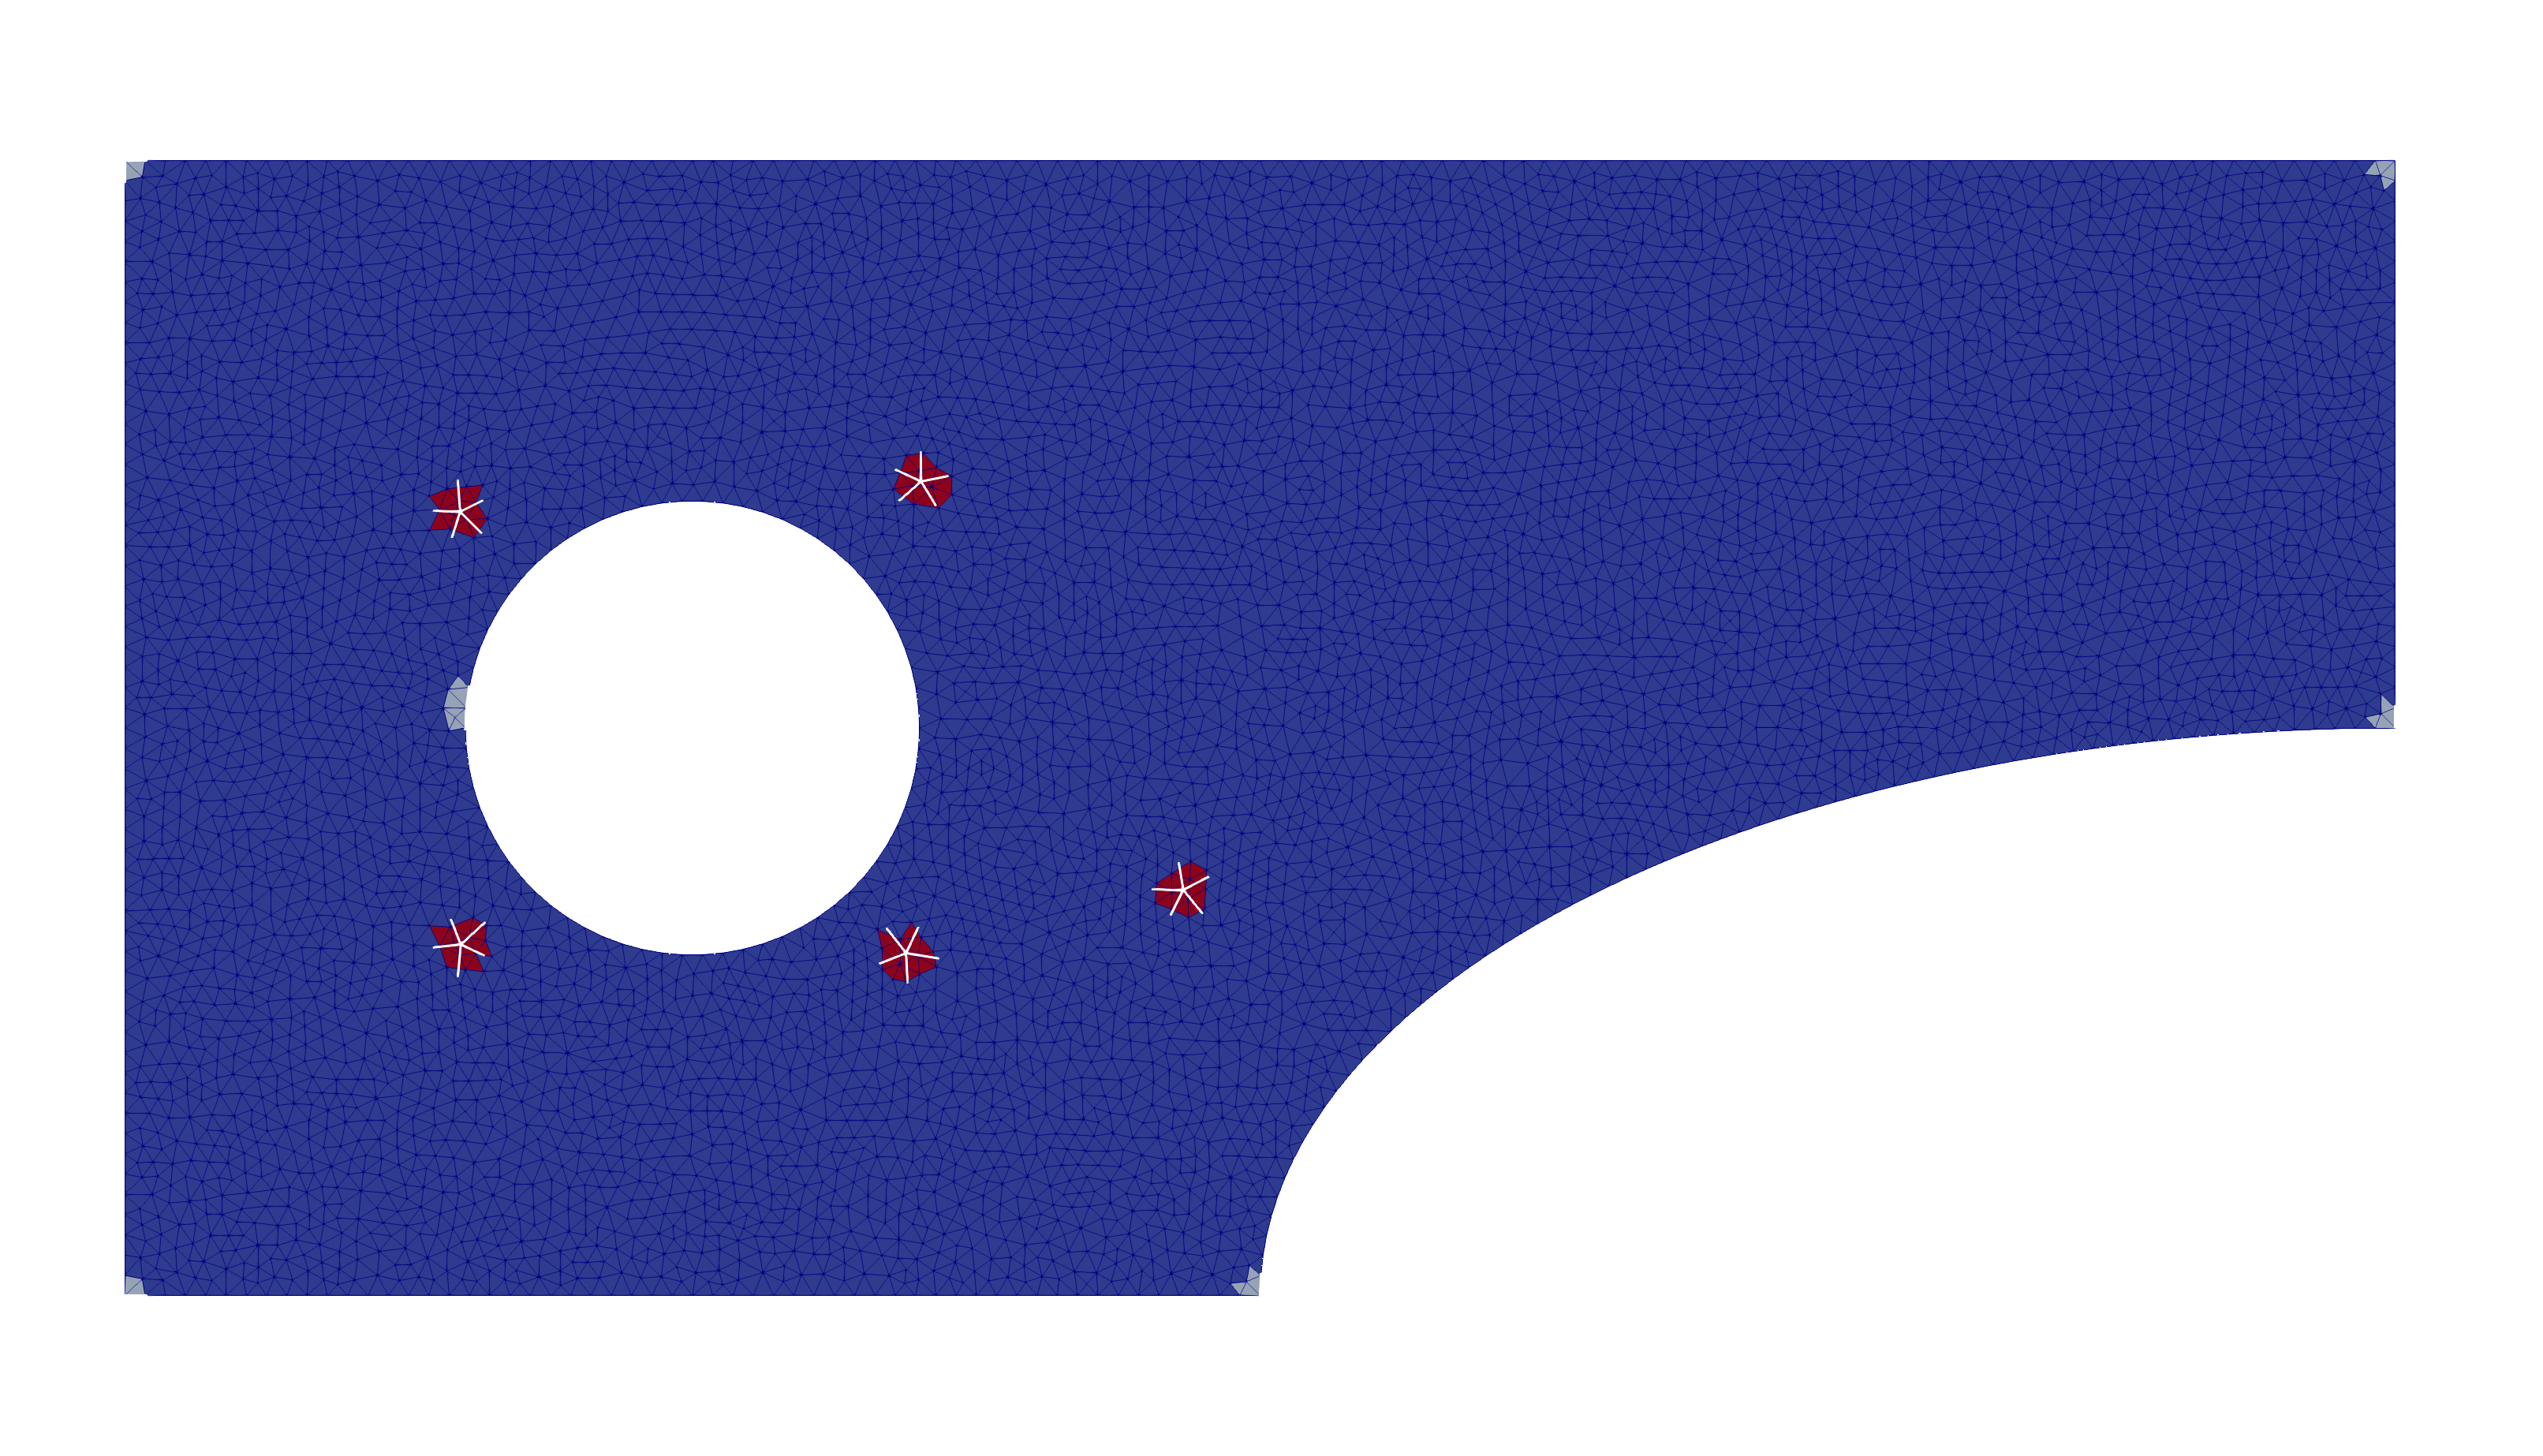
\includegraphics[height=3.7cm]{sing_slots}
%	\captionof{figure}{Simultaneous Strategy}
 %   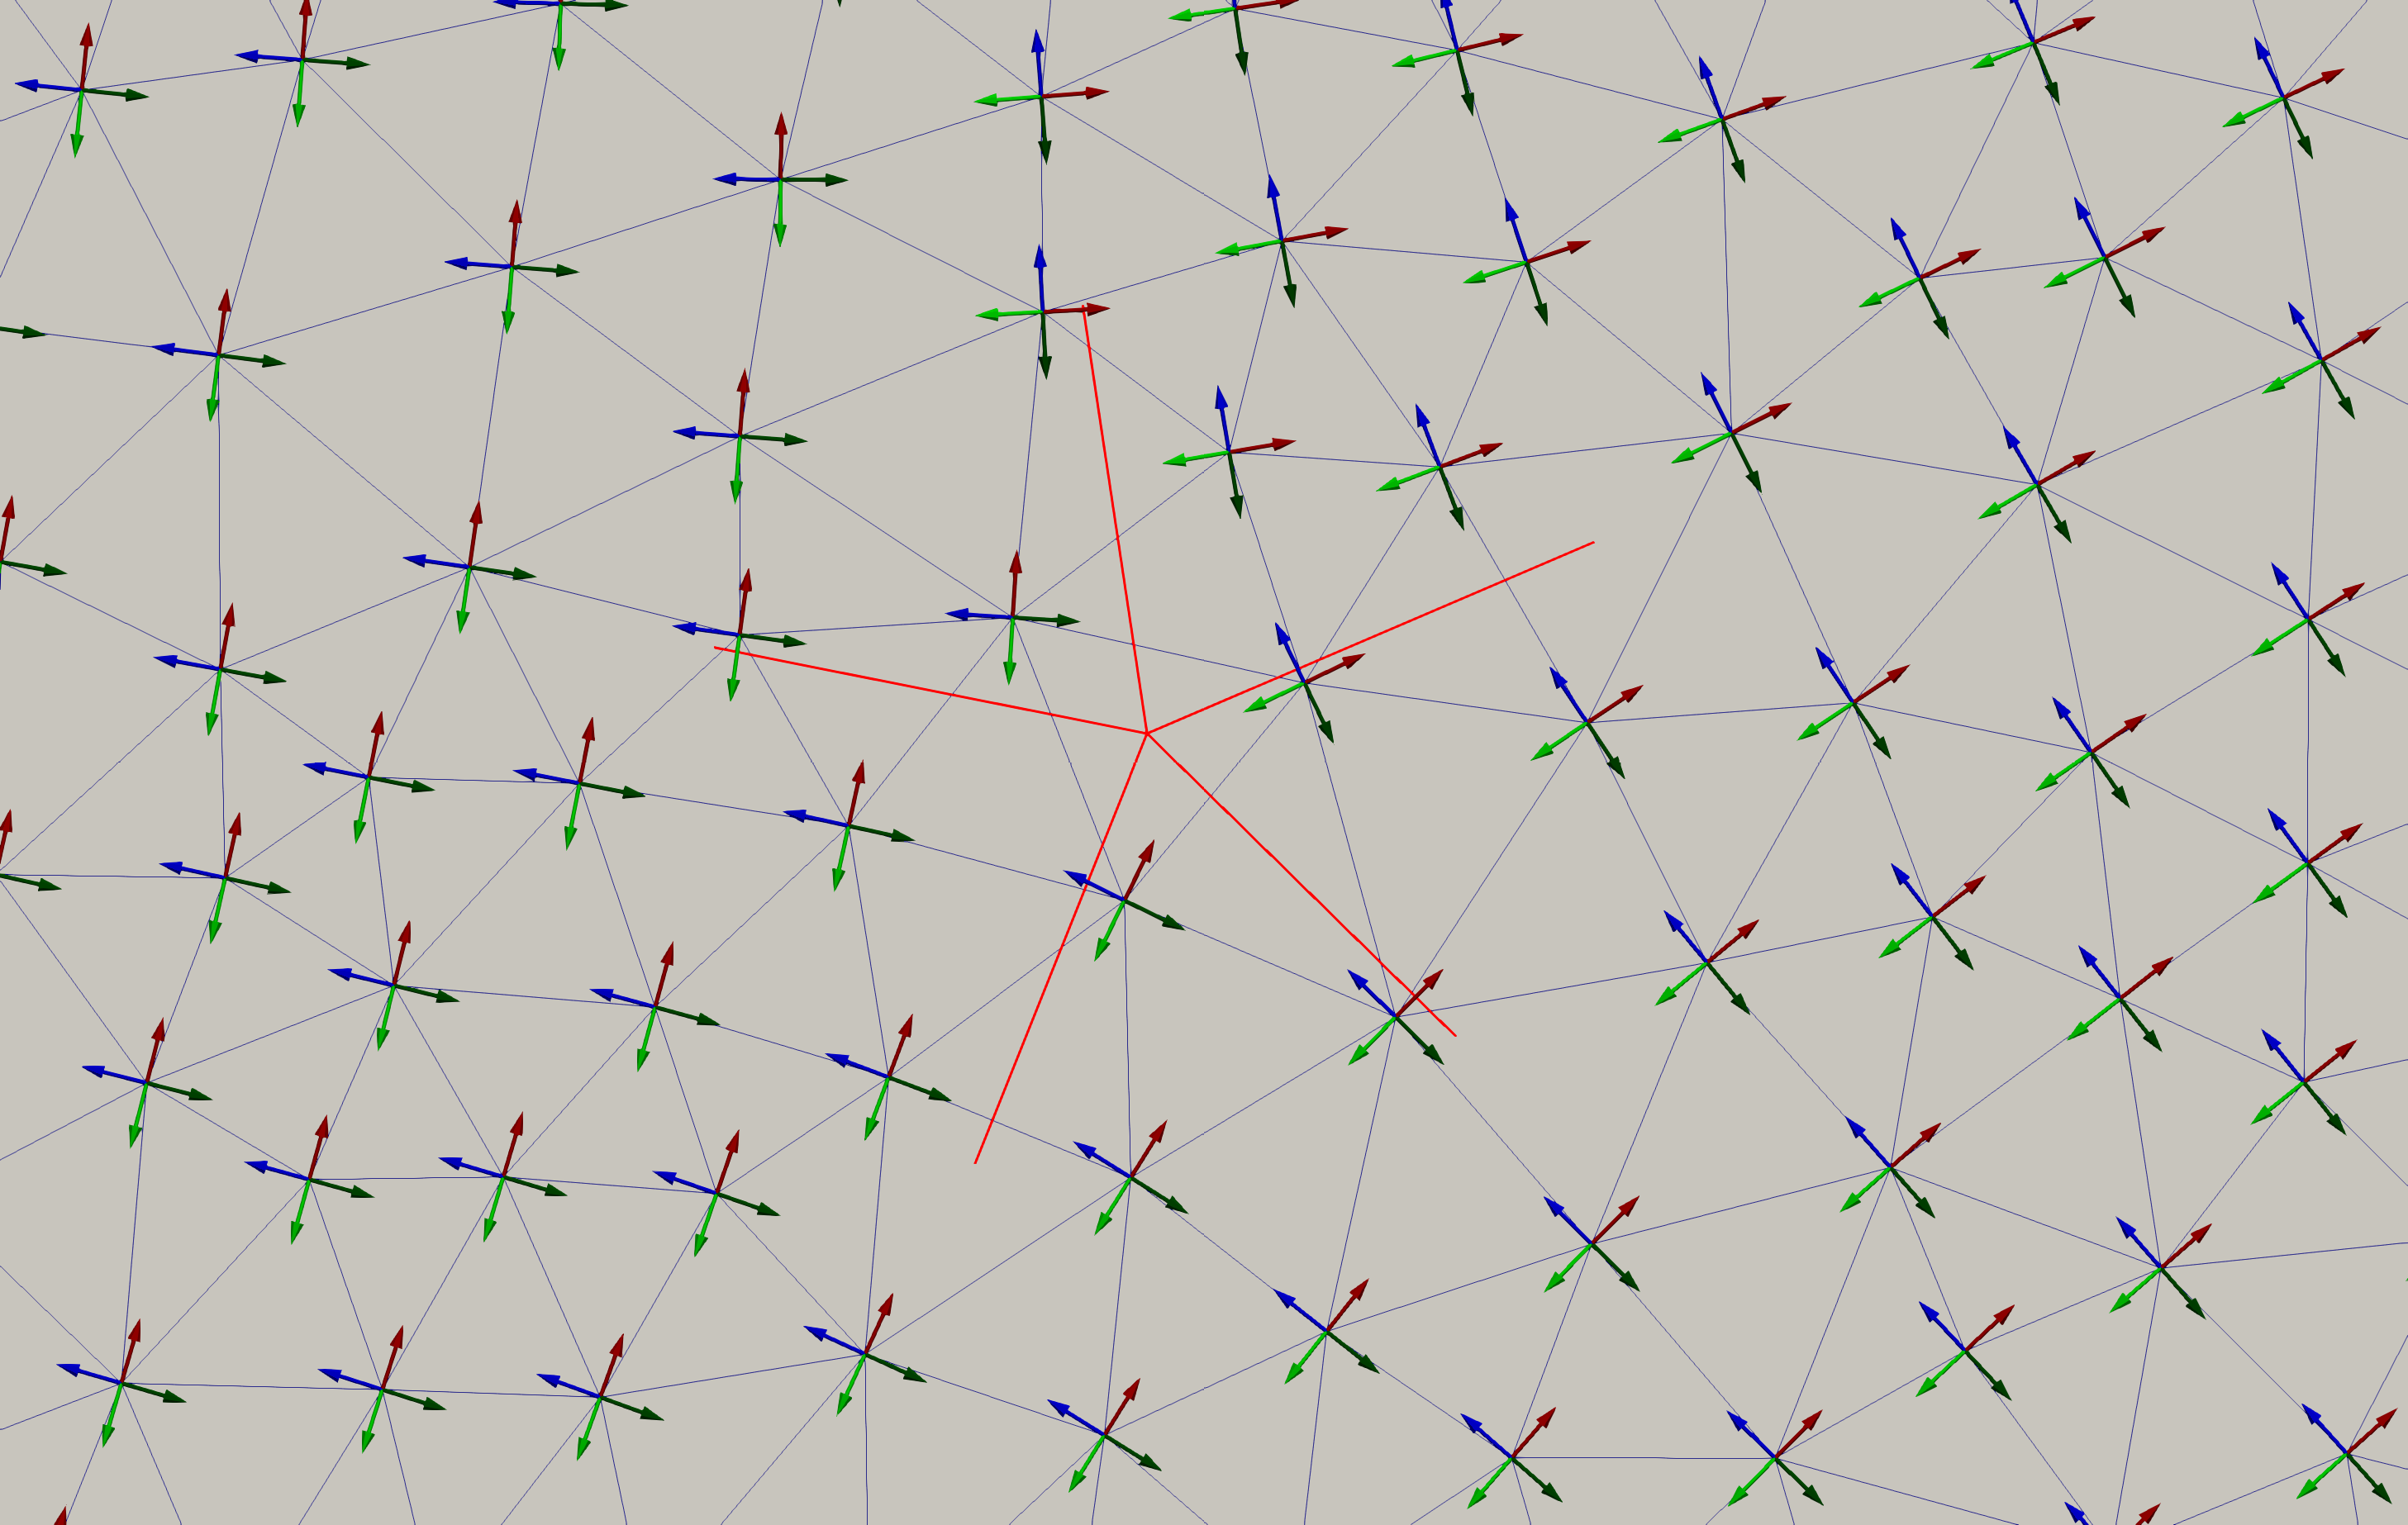
\includegraphics[height=3.7cm]{HIS-Slots-close-up}
  %  \captionof{figure}{Simultaneous Strategy}
   %% 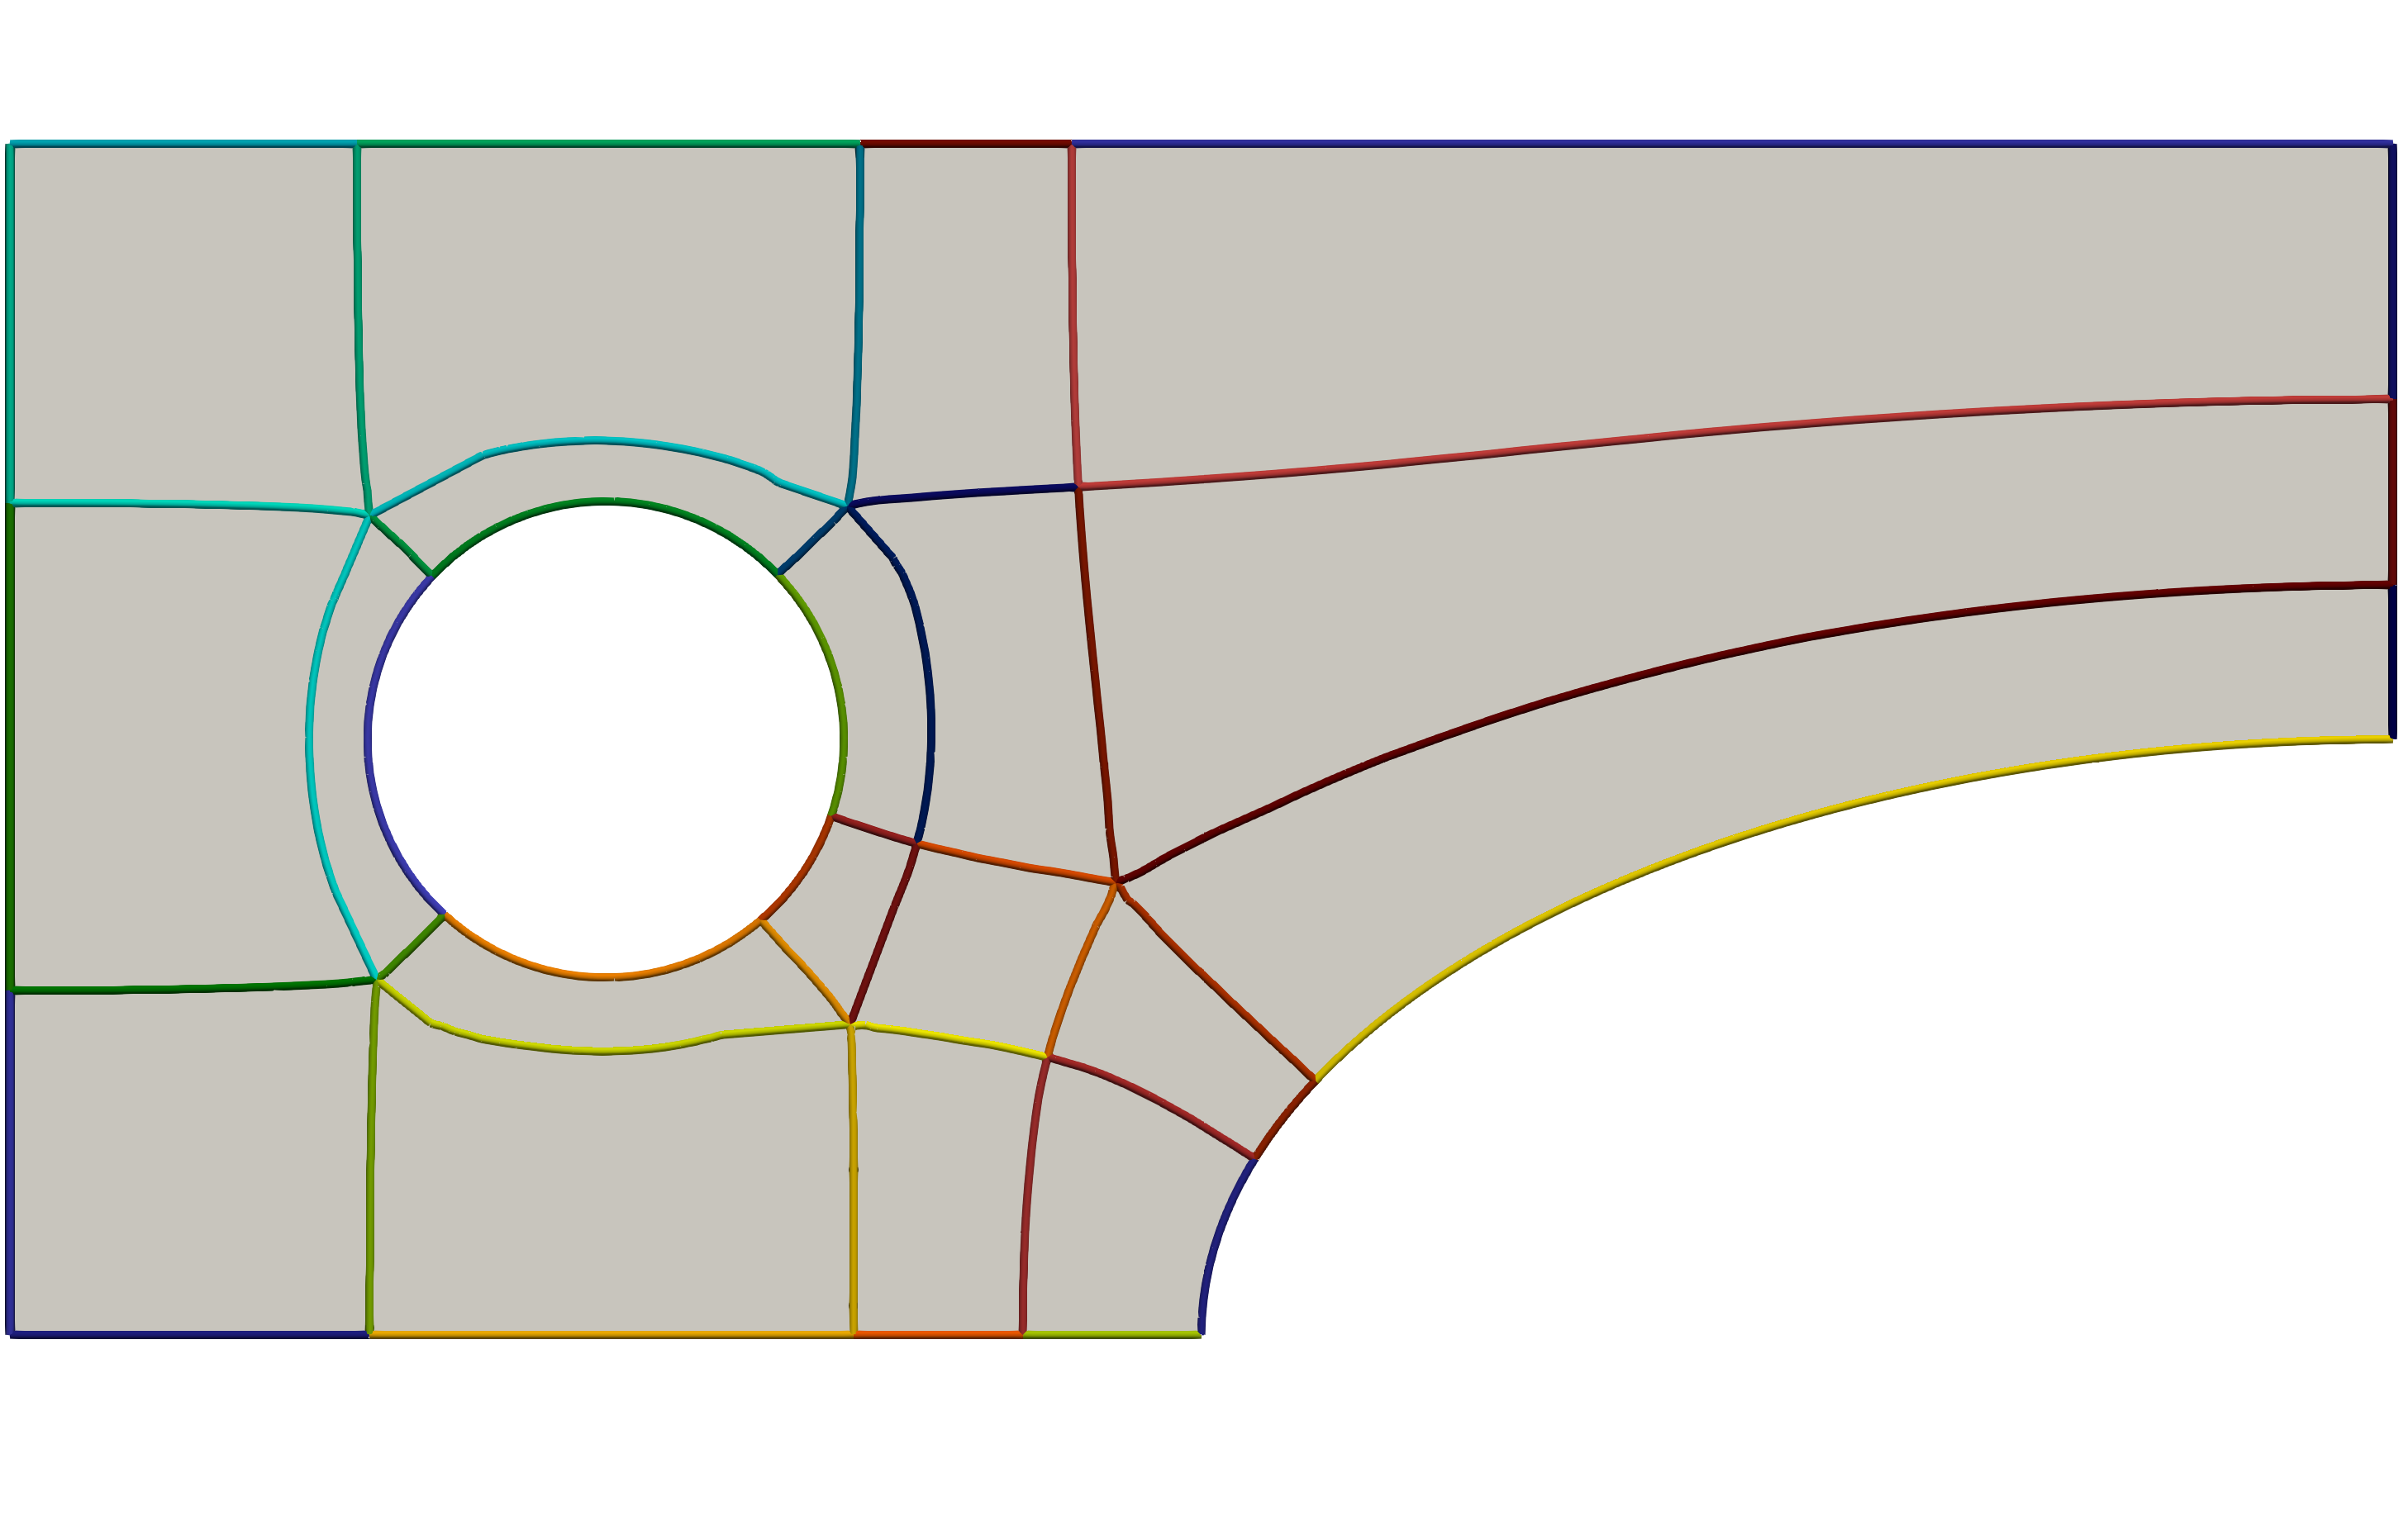
\includegraphics[height=3.7cm]{HIS-SingGraphOriginal-ConfusBallRad005}
  %  \captionof{figure}{Simultaneous Strategy}
  %  \hfill
%\includegraphics[scale=0.05]{fleche}
%\hfill
%\end{comment}
\captionsetup{width=0.2\linewidth}

   % 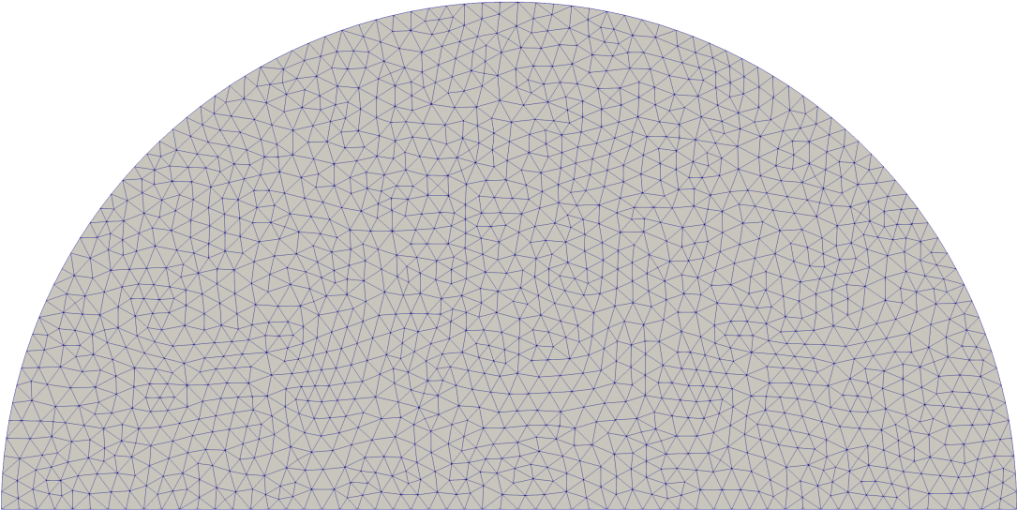
\includegraphics[width=0.2\linewidth]{1}
    %\captionof{figure}{Caption A}


\captionsetup{labelformat=empty}


\begin{minipage}[b]{0.23\linewidth}
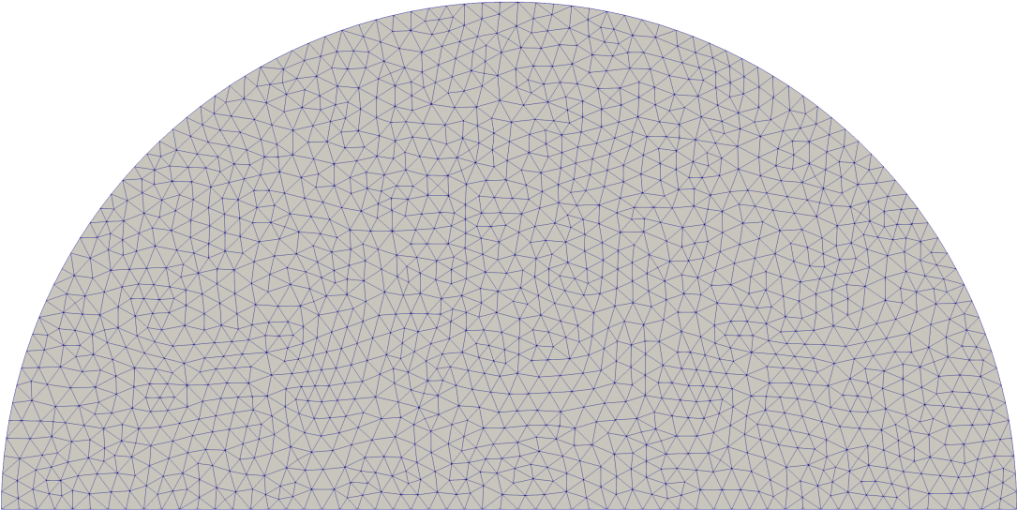
\includegraphics[width=\textwidth]{1}
\captionof{figure}{Given a triangular mesh}
\label{fig:figure1}
\end{minipage}
\hspace{0.15cm}
\begin{minipage}[b]{0.23\linewidth}

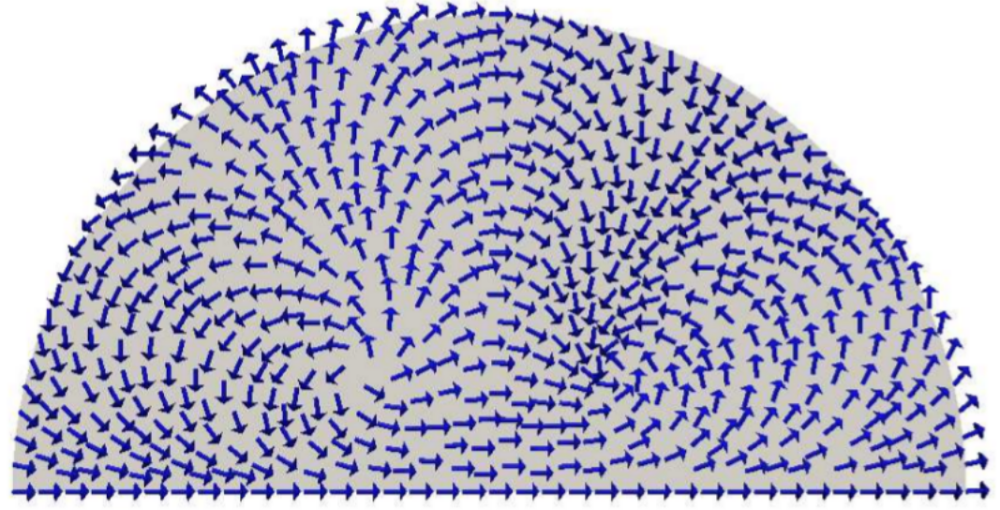
\includegraphics[width=\textwidth]{2}
\captionof{figure}{Contruct the cross-field (CF)}
\label{fig:figure2}
\end{minipage}
%%%%%%%%%%%%%%%%%%%%%%%%%%%%%%%%
\hspace{0.15cm}
\begin{minipage}[b]{0.23\linewidth}

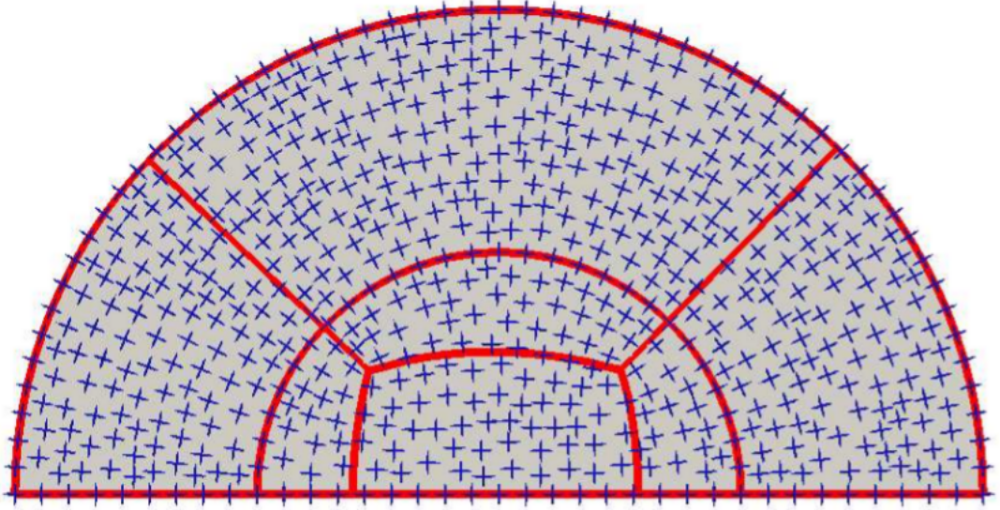
\includegraphics[width=\textwidth]{3}
\captionof{figure}{Construct the Singularity Graph}
\label{fig:figure3}
\end{minipage}
%%%%%%%%%%%%%%%%%%%%%%%%%%%%%%%%%%%%
\hspace{0.15cm}
\begin{minipage}[b]{0.23\linewidth}

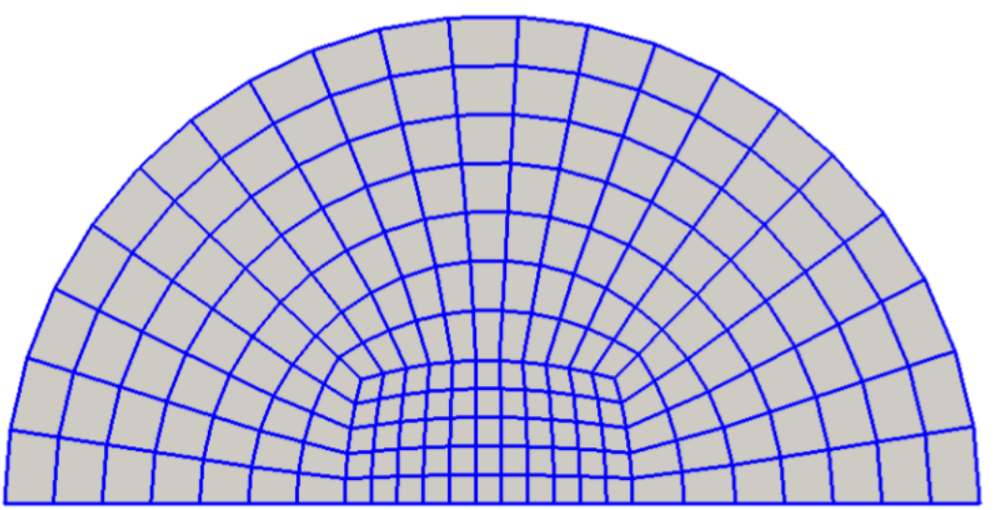
\includegraphics[width=\textwidth]{4}
\captionof{figure}{Remesh resulted quads}
\label{fig:figure4}
\end{minipage}
\bigskip

%\begin{minipage}[b]{0.99\linewidth}
%includegraphics[width=\textwidth]{Heun}
%\captionof{figure}{llustration of the integration process over a triangle}
%\label{fig:figure2}
%\end{minipage}


%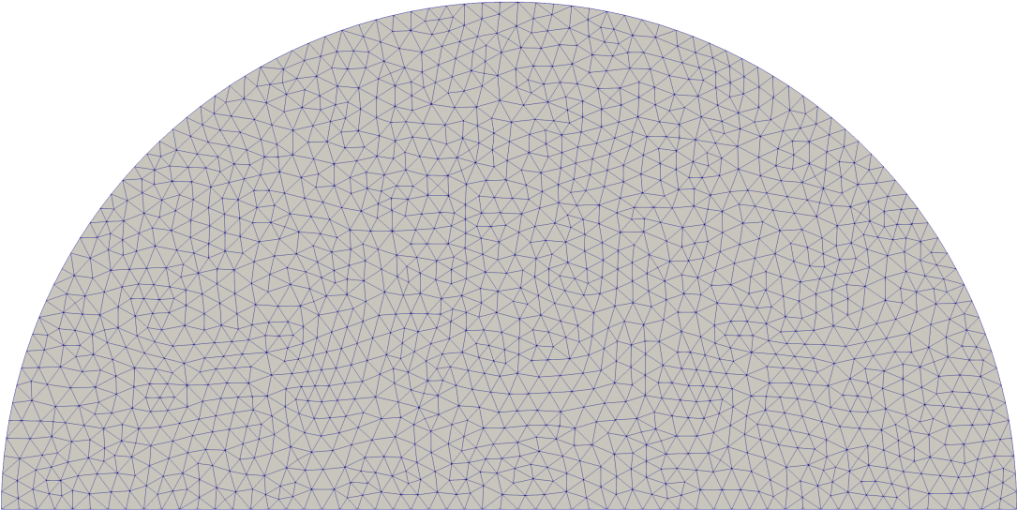
\includegraphics[height=3cm]{1}
%\captionof{figure}{Given triangular mesh}
%          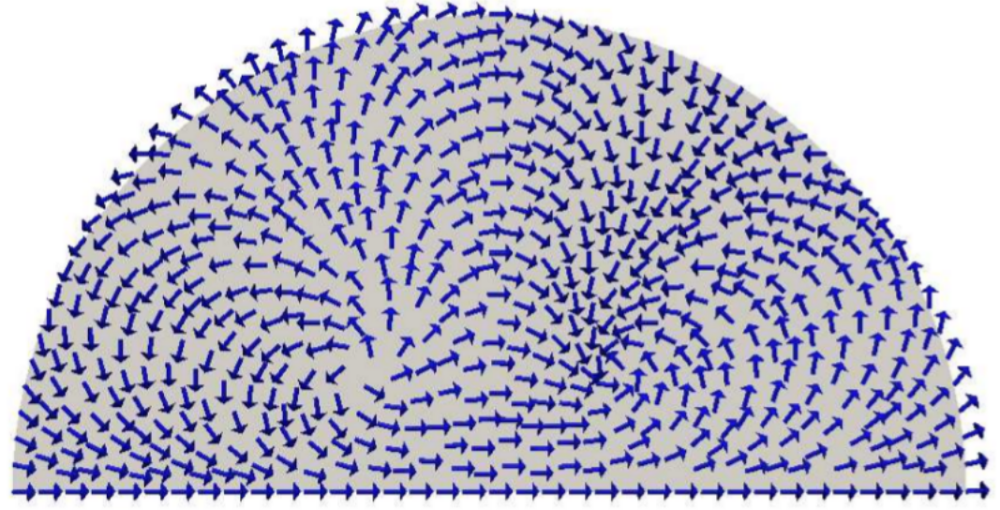
\includegraphics[height=3cm]{2}
%         \captionof{figure}{Contruct cross-field}
%          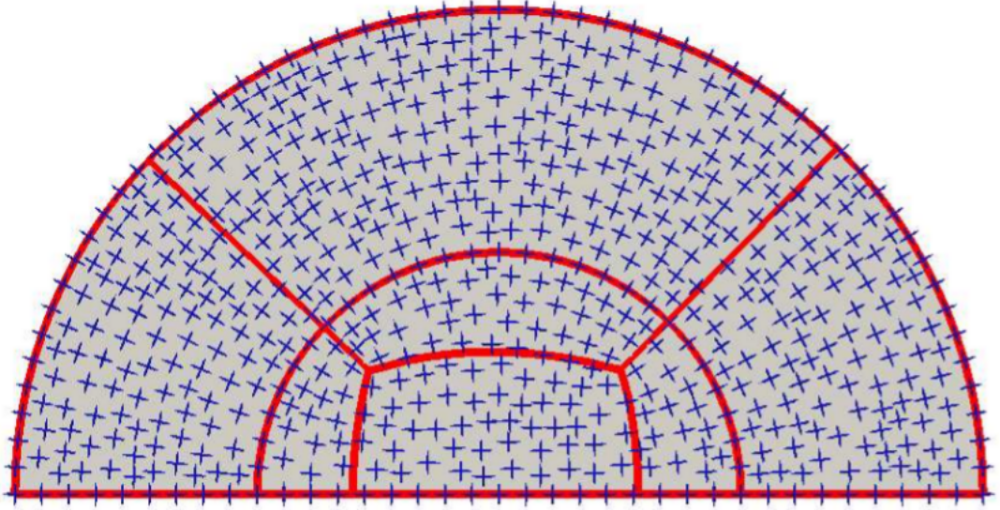
\includegraphics[height=3cm]{3}
%         \captionof{figure}{Trace separatrices of the CF}
%         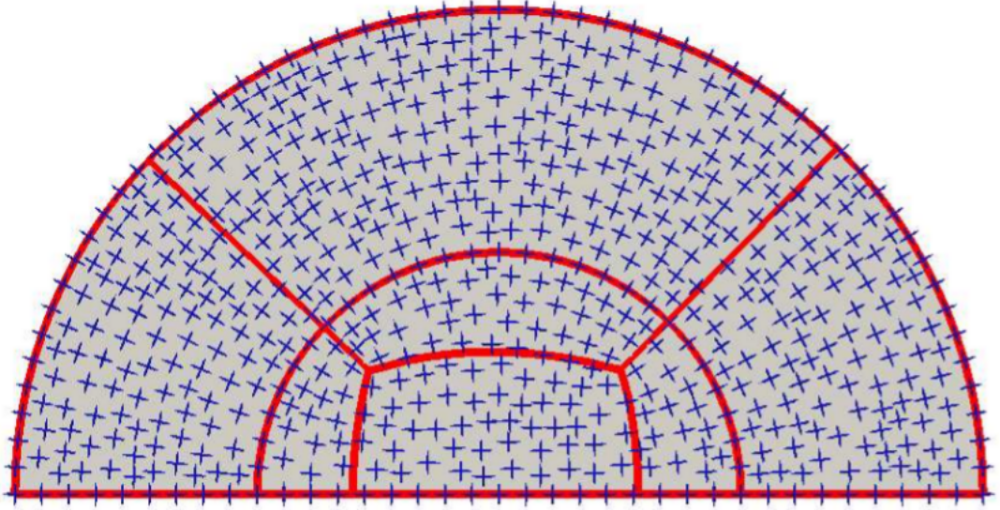
\includegraphics[height=3cm]{3}
%         \captionof{figure}{Remesh resulted quads}


}
%----------------------------------------------------------------------------------------
%	Approach
%----------------------------------------------------------------------------------------
%%%%%%%%%%%%%%%%%%%%%%%%%%%%%%%%%%%%%%%%%%%%%%%%%%%%%%%%%%%%%%%%%%%%%
\headerbox{Singularity Graph Extraction}{name=approach,column=0,row=0,below=context}{
%%%%%%%%%%%%%%%%%%%%%%%%%%%%%%%%%%%%%%%%%%%%%%%%%%%%%%%%%%%%%%%%%%%%%
\noindent
\begin{minipage}[b]{1\linewidth}
\begin{tcolorbox}[colframe=gray,boxrule=0.1pt,title=\Large $\ \ \ \ \ \ \ \ \ \ $Objectives $\ \ \ \ \  \  \ \ \ \ \ \ \ \ \ \ \ \ \ \ \ \ \ \  $Limitations]		%\begin{itemize}
	$\bullet$ Fully automatic method  $\ \ \ \ \ \ \ \ \ \ \ \ \ \ \ \ \ \ \ \ \ \bullet$  Dependence on input triangulation%	\item[$\bullet$] Fully automatic method
\newline
$\bullet$ High quality resulted quad blocks $\ \ \ \ \ \ \bullet$ Approximation errors%	\item[$\bullet$] High quality resulted quad blocks
%\end{itemize}
\end{tcolorbox}
\end{minipage}
%\vspace{0.02cm}
%\begin{minipage}[b]{0.52\linewidth}
%\begin{tcolorbox}[colframe=gray,boxrule=0.8pt,title=\Large Limitations]

%$\bullet$Approximation errors % \item[$\bullet$] Approximation errors
%\newline
%$\bullet$Dependence on input triangulation %\item[$\bullet$] Dependence on input triangulation

%\end{tcolorbox}
%\end{minipage}

}



%----------------------------------------------------------------------------------------
%	Implementation
%----------------------------------------------------------------------------------------

%%%%%%%%%%%%%%%%%%%%%%%%%%%%%%%%%%%%%%%%%%%%%%%%%%%%%%%%%%%%%%%%%%%%%
\headerbox{Strategies}{name=strategies,column=0,below=approach}{
%%%%%%%%%%%%%%%%%%%%%%%%%%%%%%%%%%%%%%%%%%%%%%%%%%%%%%%%%%%%%%%%%%%%%
\noindent
\begin{tcolorbox}[colframe=gray,boxrule=0.8pt,title=\Large Continuous Strategies]
(Iteratively/ Simultaneuously) Depart from each singular point along each
slot direction until reaching:
\newline
	%	\begin{itemize}
  $\ \ \ \ \ \ \ a)\ $ the boundary
\newline
  $\ \ \ \ \ \ \ b_1)$ the vicinity of a different singularity (confusing ball $\rightarrow$ Fig.~\ref{fig:figure5} - red circles) - \textbf{Sequential Strategy}
\newline
  $\ \ \ \ \ \ \ b_2)$ the vicinity of a different singularity line (thresholdDistance $\rightarrow$ Fig.~\ref{fig:figure6} - red circles) - \textbf{Simultaneous Strategy}		
	\end{tcolorbox}
\captionsetup{labelformat=empty}
\noindent
\begin{minipage}[b]{0.49\linewidth}
\includegraphics[width=\textwidth]{HIS4-orig-Rad003}
\captionof{figure}{Sequential Strategy}
\label{fig:figure5}
\end{minipage}
\hspace{0.005\linewidth}
\begin{minipage}[b]{0.49\linewidth}
\includegraphics[width=\textwidth]{HIS4-sim-Rad003}
\captionof{figure}{Simultaneous Strategy}
\label{fig:figure6}
\end{minipage}

\vspace{0.15cm}%
\noindent
\begin{minipage}[!Ht]{0.49\linewidth}
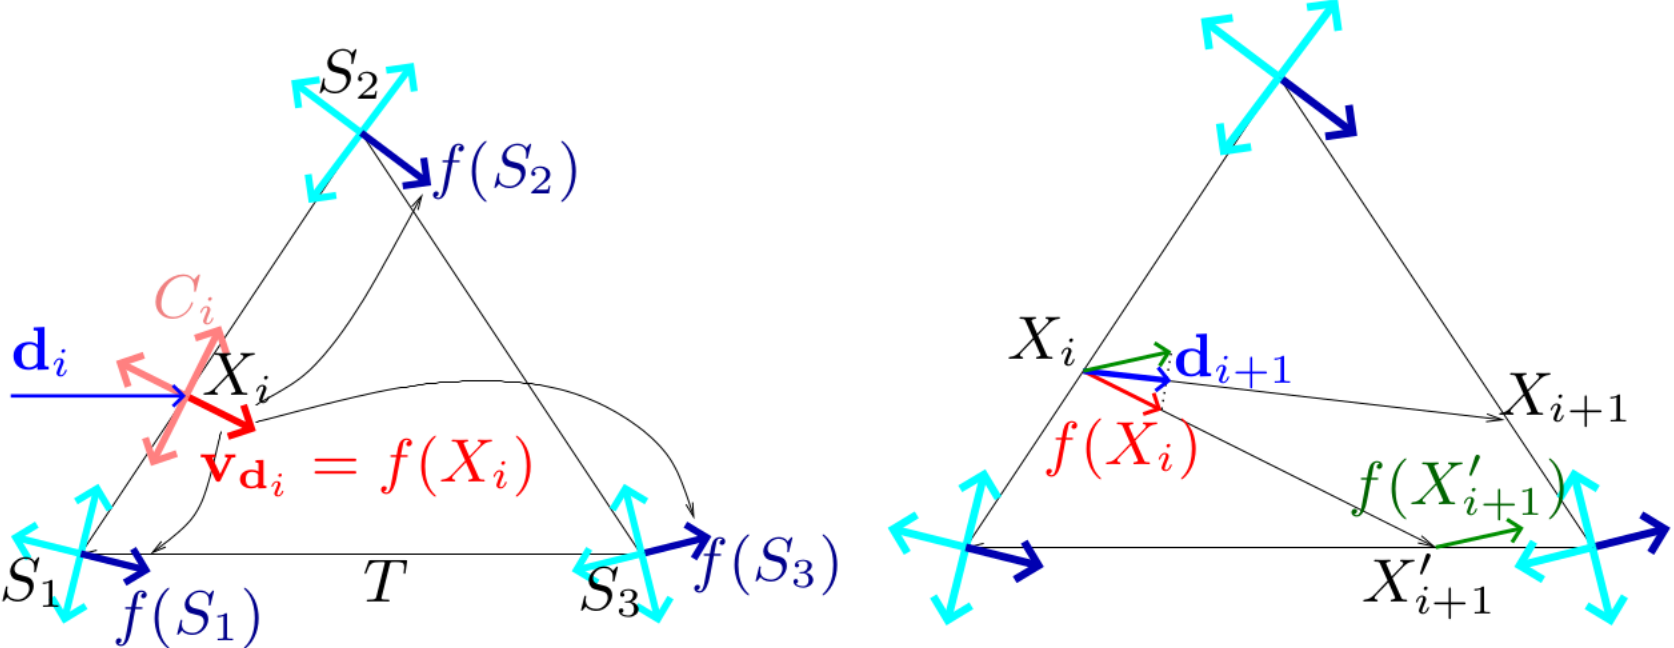
\includegraphics[width=\textwidth]{Heun}
\captionof{figure}{Illustration of the integration process (Heun) over a triangle}
\label{fig:figure7}
\end{minipage}
\hspace{0.005\linewidth}
\begin{minipage}[!Ht]{0.49\linewidth}
\includegraphics[width=\textwidth]{SingZoom}
\captionof{figure}{Singularities and slots (left - degree 3, right - degree 5)}
\label{fig:figure8}
\end{minipage}

%\newline	
\bigskip
%\vspace{0.5cm}
\noindent
\begin{minipage}[!Ht]{0.49\linewidth}
 \textbf{Challenges}
\newline	
\medskip

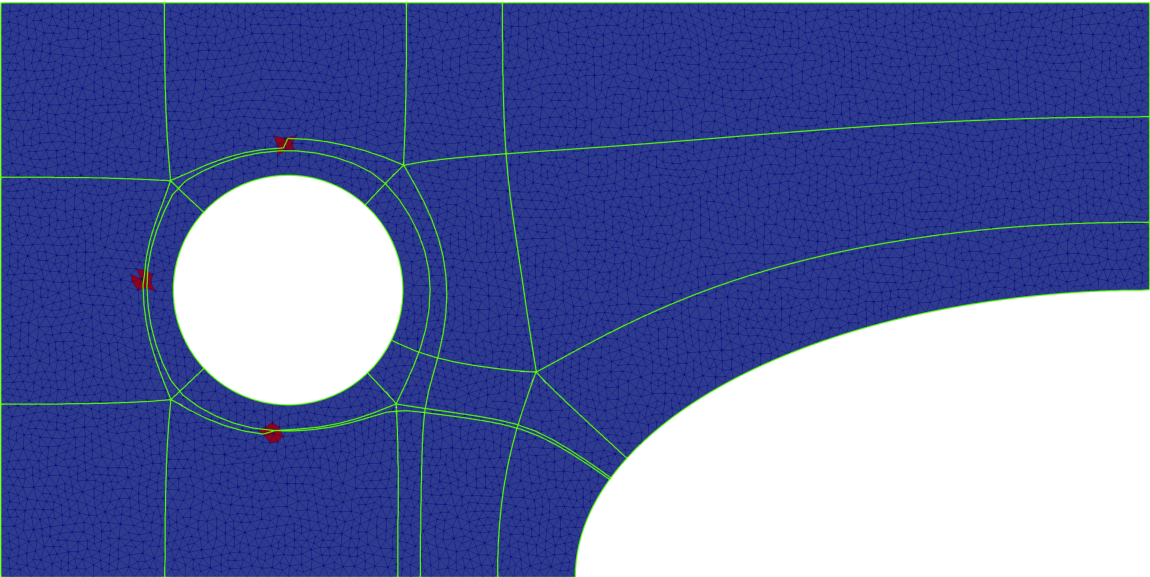
\includegraphics[width=\textwidth]{HIS4-sim-Rad002}
\captionof{figure}{ a) "miss the connection"}
\label{fig:figure9}

\bigskip
b) dependence on proximity parameter - confusing ball radius, thresholdDistance

\bigskip
\end{minipage}
%\vspace{-3cm}
\hspace{0.005\linewidth}
\begin{minipage}[!Ht]{0.48\linewidth}
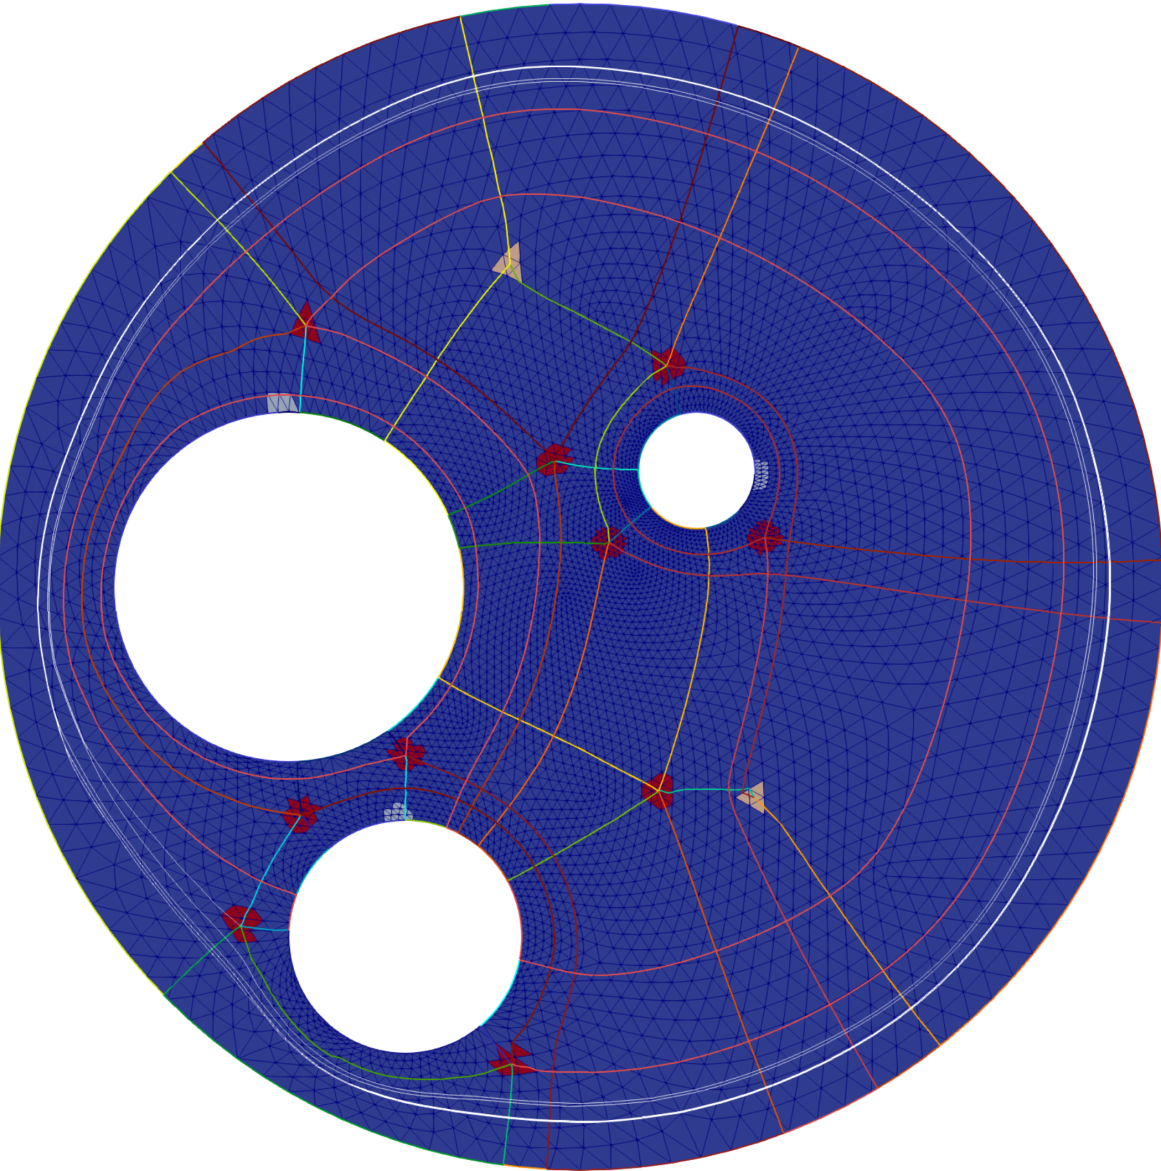
\includegraphics[width=\textwidth]{Circle_with_circle_holes_refSS1-cycle}
\captionof{figure}{ c) Cycles}
\label{fig:figure10}
\end{minipage}
%%%%%%%%%%%%%%%%%%%	
%
%\begin{minipage}[b]{0.5\linewidth}%\begin{flushleft}
%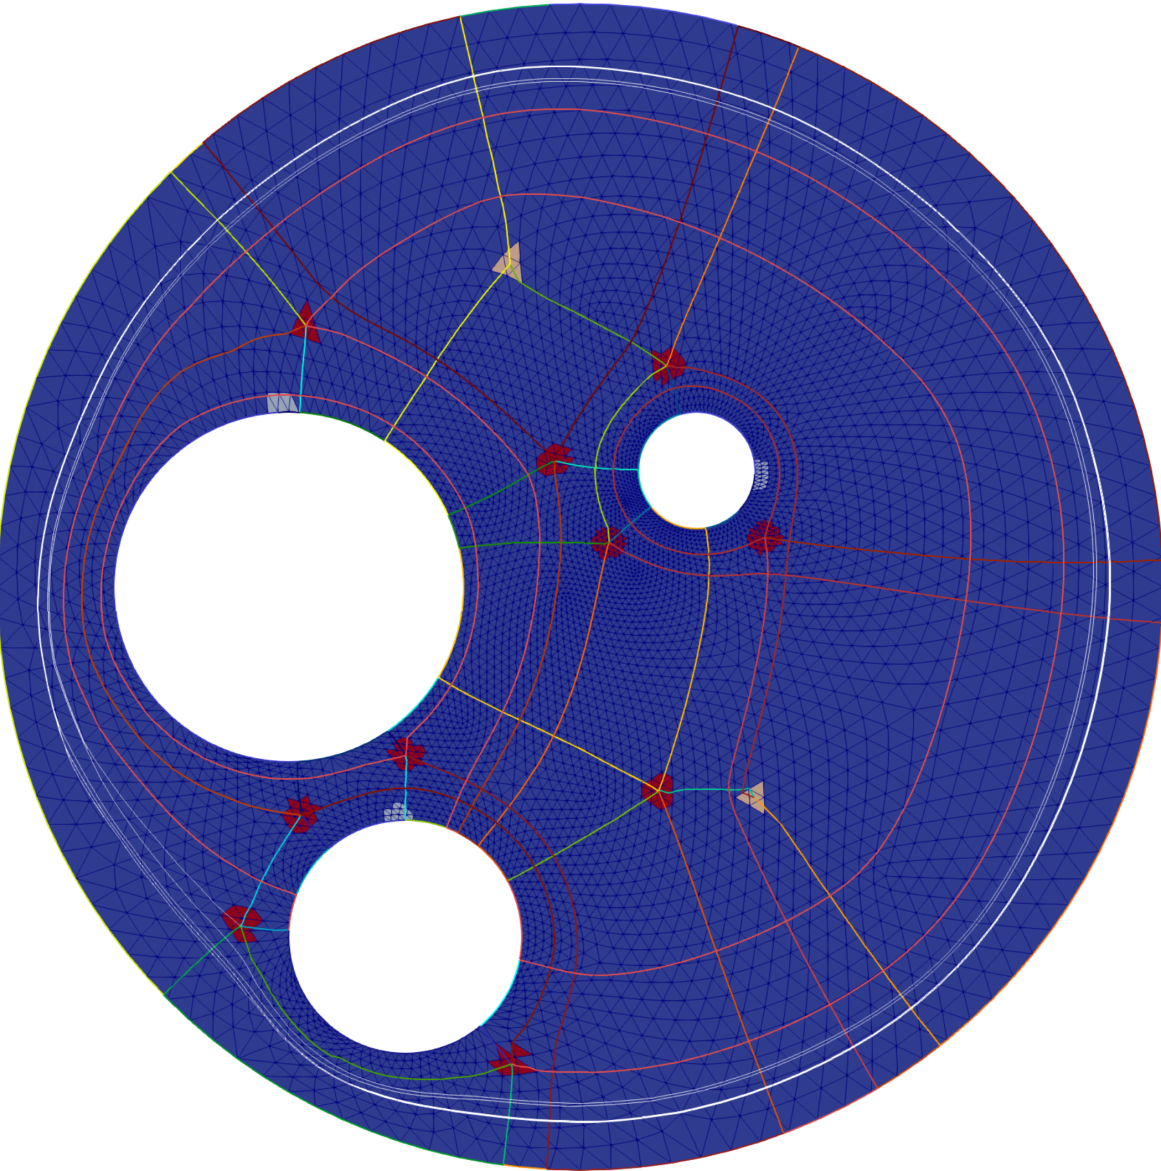
\includegraphics[width=\textwidth]{Circle_with_circle_holes_refSS1-cycle}
%\captionof{figure}{ a) Cycles}
%\label{fig:figure2}%\end{flushleft}
%\end{minipage}
%\vspace{0.05\linewidth}
%\begin{minipage}[b]{0.49\linewidth}%\begin{flushright}
%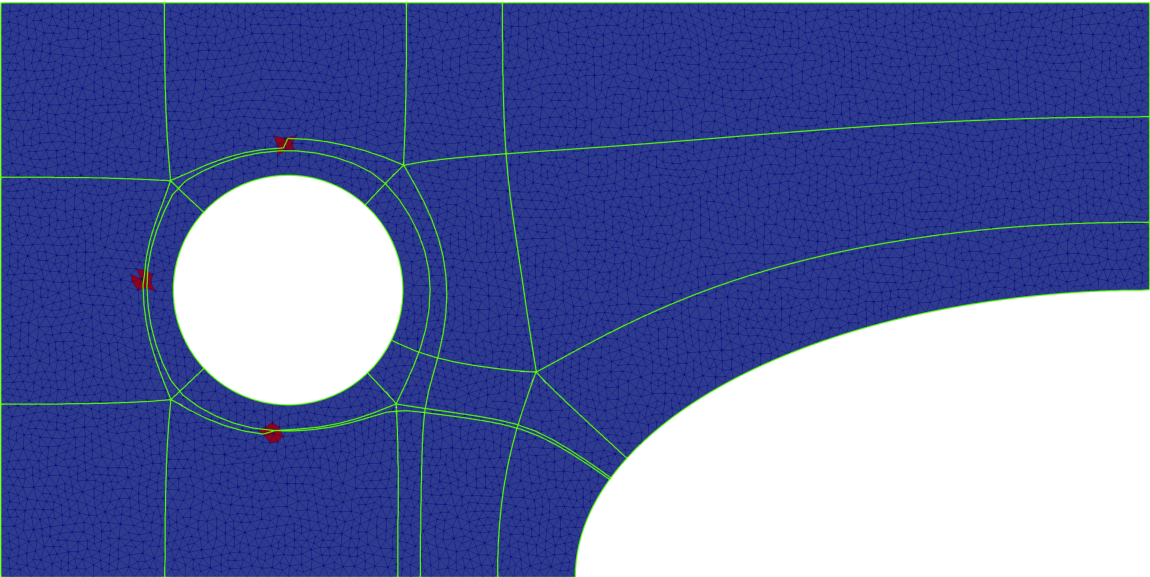
\includegraphics[width=\textwidth]{HIS4-sim-Rad002}
%\captionof{figure}{ b) "miss the connection"}
%\label{fig:figure2}
%	\bigskip
%	
%$c)$ dependence on proximity parameter - confusing ball radius, thresholdDistance
%
%%%%\end{flushright}
%\end{minipage}
%\bigskip
}

%--------------------------------------------------------------------------------------------

%\headerbox{}%
%{name=foottext, column=0, above=bottom, textborder=none, headerborder=none, boxheaderheight=0pt}{
%\noindent JOURNEE DES THESARDS ET DES POST DOC.\indent  June 19, France

%}



  %----------------------------------------------------------------------------------------
%	Experimentation
%----------------------------------------------------------------------------------------
%%%%%%%%%%%%%%%%%%%%%%%%%%%%%%%%%%%%%%%%%%%%%%%%%%%%%%%%%%%%%%%%%%%%%
\headerbox{Strategies}{name=experimentation,column=1,below=context}{
%%%%%%%%%%%%%%%%%%%%%%%%%%%%%%%%%%%%%%%%%%%%%%%%%%%%%%%%%%%%%%%%%%%%%
\begin{tcolorbox}[colframe=gray,boxrule=0.8pt,title=\Large Discrete Strategy]
Build a meta-graph of shortest paths, using a modified Dijkstra's algorithm
\newline

\begin{minipage}[b]{0.455\linewidth}%\begin{flushleft}
\textbf{Advantages}
\newline
\medskip%\begin{itemize}
$\bullet$ No infinite cycles
\newline
$\bullet$ All possible connections - a matter of choice
\end{minipage}
\vspace{0.05\linewidth}
\begin{minipage}[b]{0.455\linewidth}	%\begin{flushright}
\textbf{Limitations}
\newline
\medskip
$\bullet$ Depends on the mesh resolution
\newline
$\bullet$ Computationally expensive
\newline
\end{minipage}
\vspace{-0.6cm}
\end{tcolorbox}
\captionsetup{labelformat=empty}
%%%%%%%%%%%%%%%%%%%%%%%%%%%%%%%%%%%%%%%%%%%%%%%%%%%%%%
\noindent
\begin{minipage}[b]{0.53\linewidth}%\begin{flushleft}
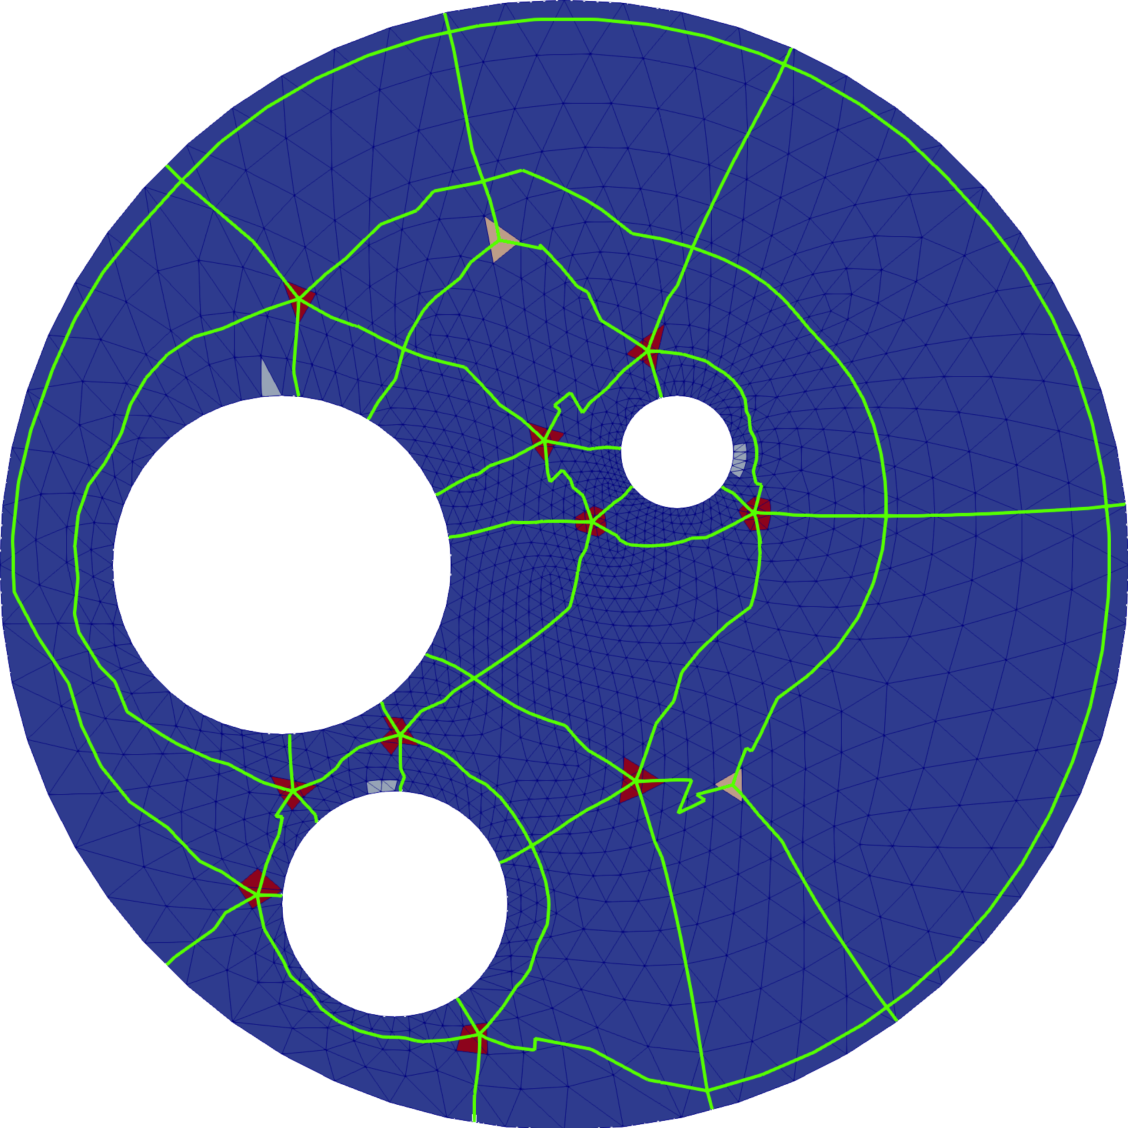
\includegraphics[width=\textwidth]{CWCH_coarse-shortest_paths}%\end{flushleft}
\captionof{figure}{Discrete Strategy - No cycles}
\vspace{0.57cm}	
\textbf{Algorithm - shortest paths}
 \begin{flushleft} 
	\begin{algorithmic}[1]
\State $dist[source]\gets 0;$
\While{$Q\not=\emptyset$}
\State $u:= center\ of\ triangle\ in\ Q;$
\State $Q\gets Q\setminus u;$
\If{$u\in Targets$}
\State{$dist[u] = dist[u] + w\_penalty * \angle(CT_{previous}[u] -CT_{target\_slot\_u});$}
\State{$return\ u;$}
\EndIf
\For{$v\in Neigh(u); v\ not\ visited$}
\State $\widetilde{CT_v}\gets closest\ {CT_v}\ w.r.t\ \widetilde{CT_u};$
\State $dist_{temp}\gets dist[u] + w\_penalty * \angle(\widetilde{CT_u}, \widetilde{CT_v}) + \angle(\widetilde{CT_v}, \overrightarrow{uv});$
\If{$dist_{temp} < dist[v]$}
\State $dist[v]\gets dist_{temp};$
\State $previous[v] = u;$
\State $CT_{previous}[v] = \widetilde{CT_v};$
\EndIf
\EndFor
\EndWhile
\end{algorithmic}
\end{flushleft}
\end{minipage}
\vspace{0.05\linewidth}
\begin{minipage}[b]{0.465\linewidth}	%\begin{flushright}
\includegraphics[width=\textwidth]{HIS3-shortest_paths}
\captionof{figure}{Discrete Strategy - $|T| = 7219$}
\label{fig:figure11}	 
\vspace{0.2cm}	
\includegraphics[width=\textwidth]{HIS6-shortest_paths}
\captionof{figure}{Discrete Strategy - $|T| = 102707$}
\label{fig:figure12}	%\end{flushright}
\vspace{0.2cm}	
 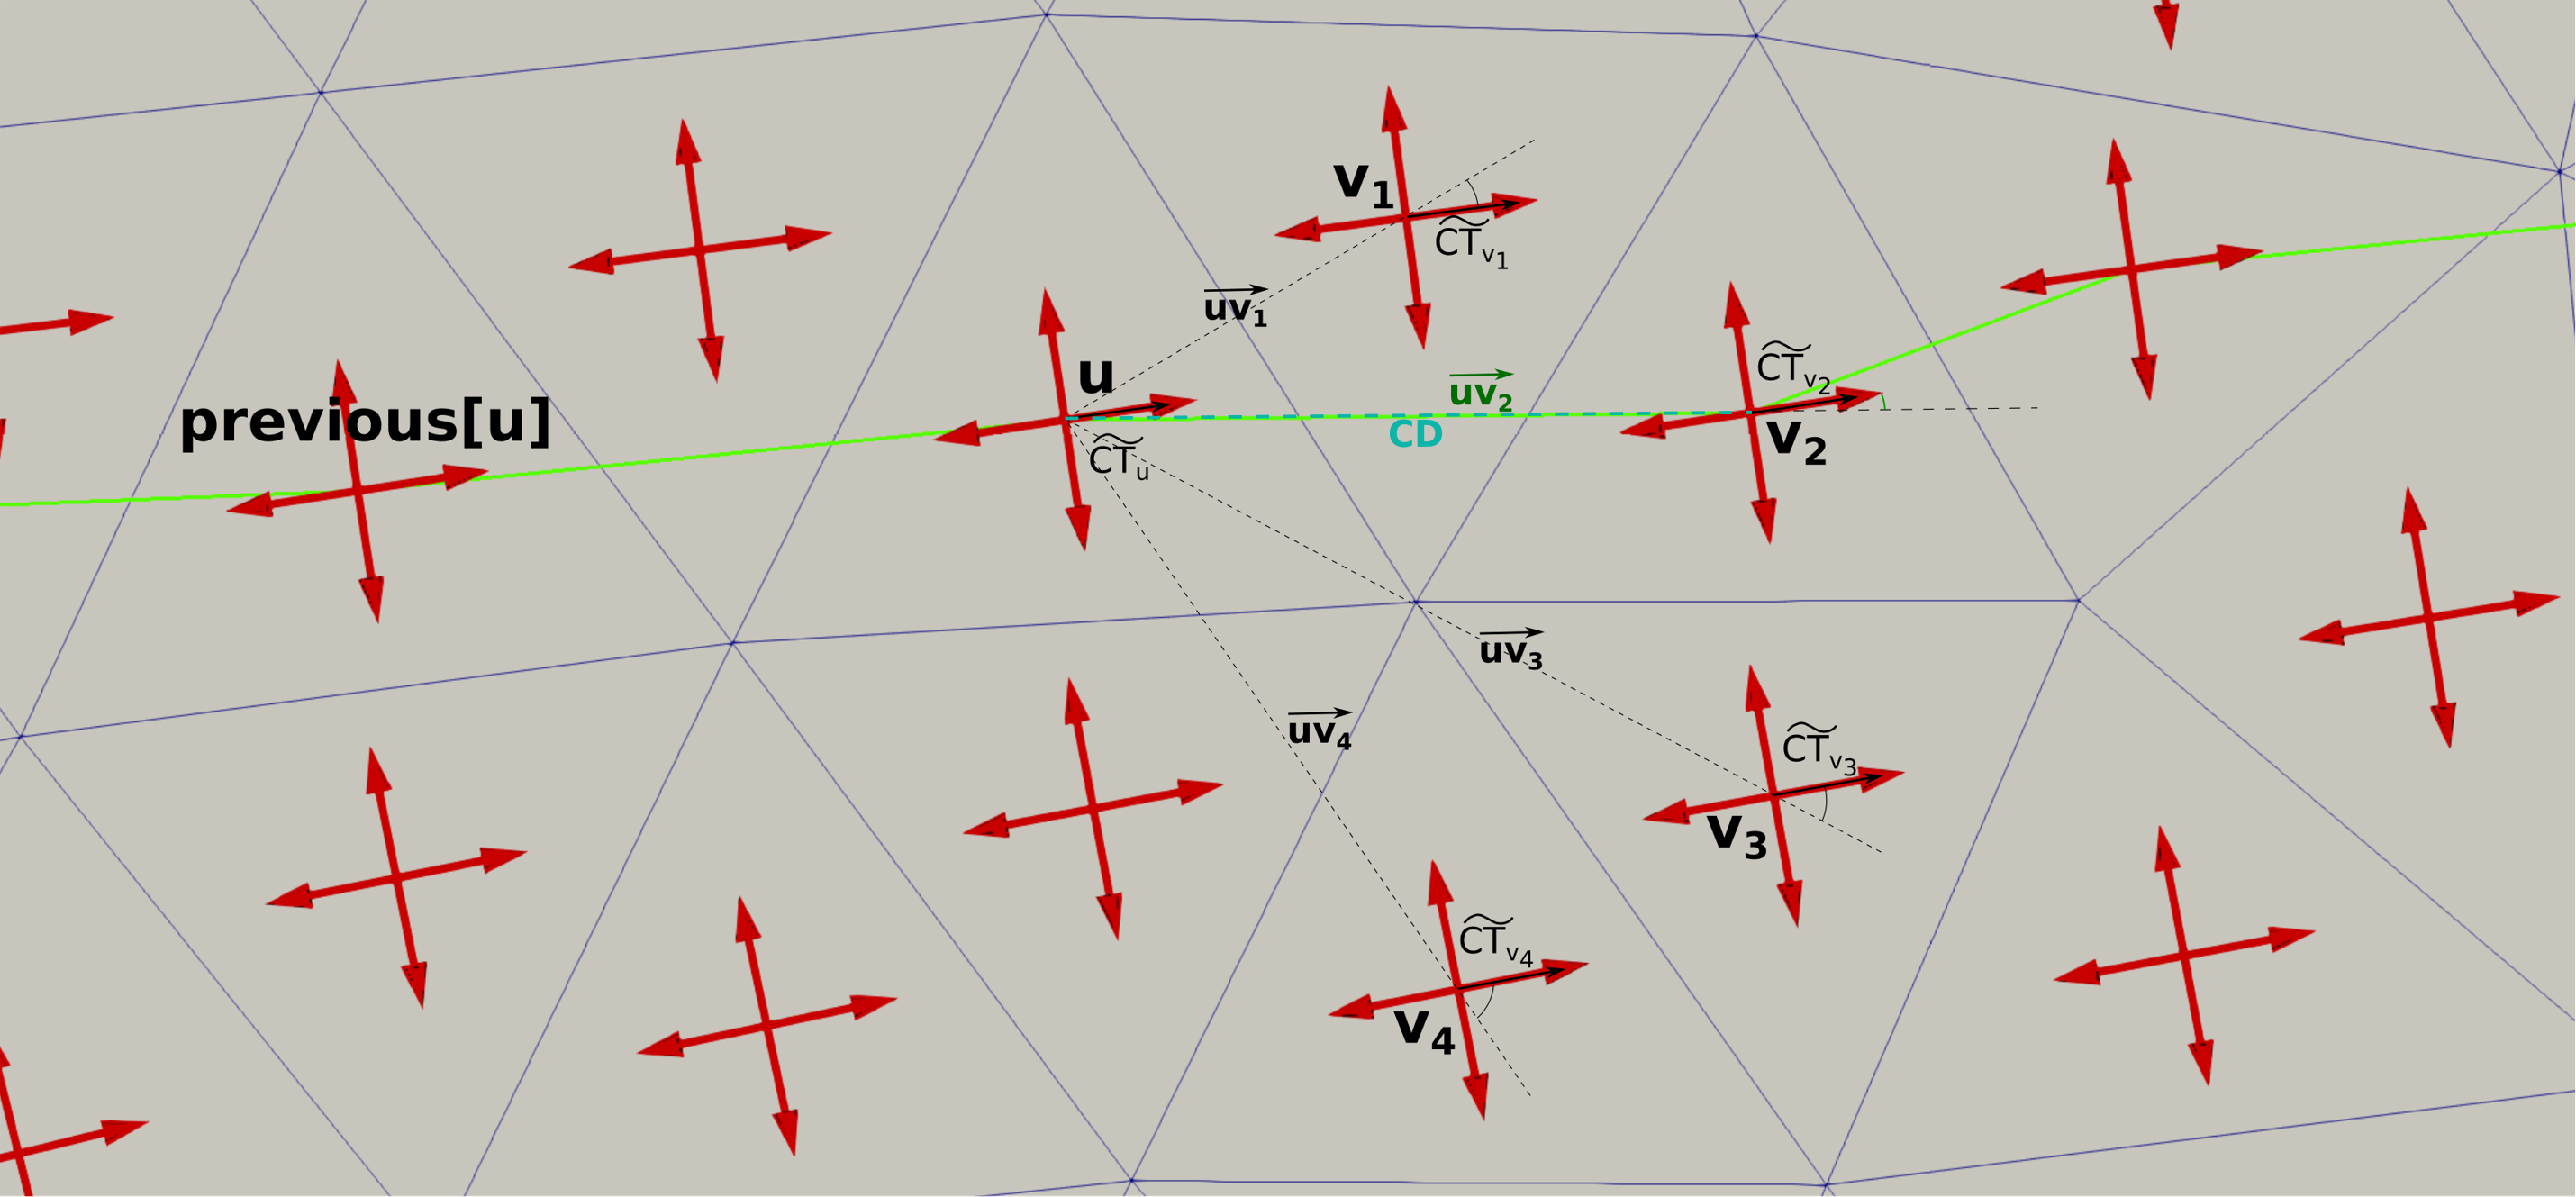
\includegraphics[width=\textwidth]{shortestPaths-zoom2}
	%\begin{minipage}[b]{1.0\linewidth}	
	%\raisebox{-\height+0.7\baselineskip}{\includegraphics[width=\linewidth]{HIS4-shortest_paths}}
	%\captionof{figure}{Weights: $\angle(CT_0, CT_1) + \angle(CT_0, \overrightarrow{T_0T_1})$}
	\label{fig:figure1}	
	
	$\bullet$ Starting from a triangle slot - $source$
	\newline

	$\bullet$ Walk along triangle centers $(u, v_0, v_1...)$, visiting adjacent triangles $(Neigh)$	
\newline	

	$\bullet$ Distance as the angle difference between the (previous and current ) crosses and between the geometric direction ($\overrightarrow{uv}$) and the previous cross
	\newline
	
	$\bullet$ Get the shortest paths towards the slots of other singularities (or boundary) - $Targets$
\end{minipage}
}
%----------------------------------------------------------------------------------------
%	Results
%----------------------------------------------------------------------------------------
%%%%%%%%%%%%%%%%%%%%%%%%%%%%%%%%%%%%%%%%%%%%%%%%%%%%%%%%%%%%%%%%%%%%%
%\headerbox{Results}{name=results,column=1,below=experimentation}{
%%%%%%%%%%%%%%%%%%%%%%%%%%%%%%%%%%%%%%%%%%%%%%%%%%%%%%%%%%%%%%%%%%%%%
%\captionsetup{labelformat=empty}
%\begin{center}
%	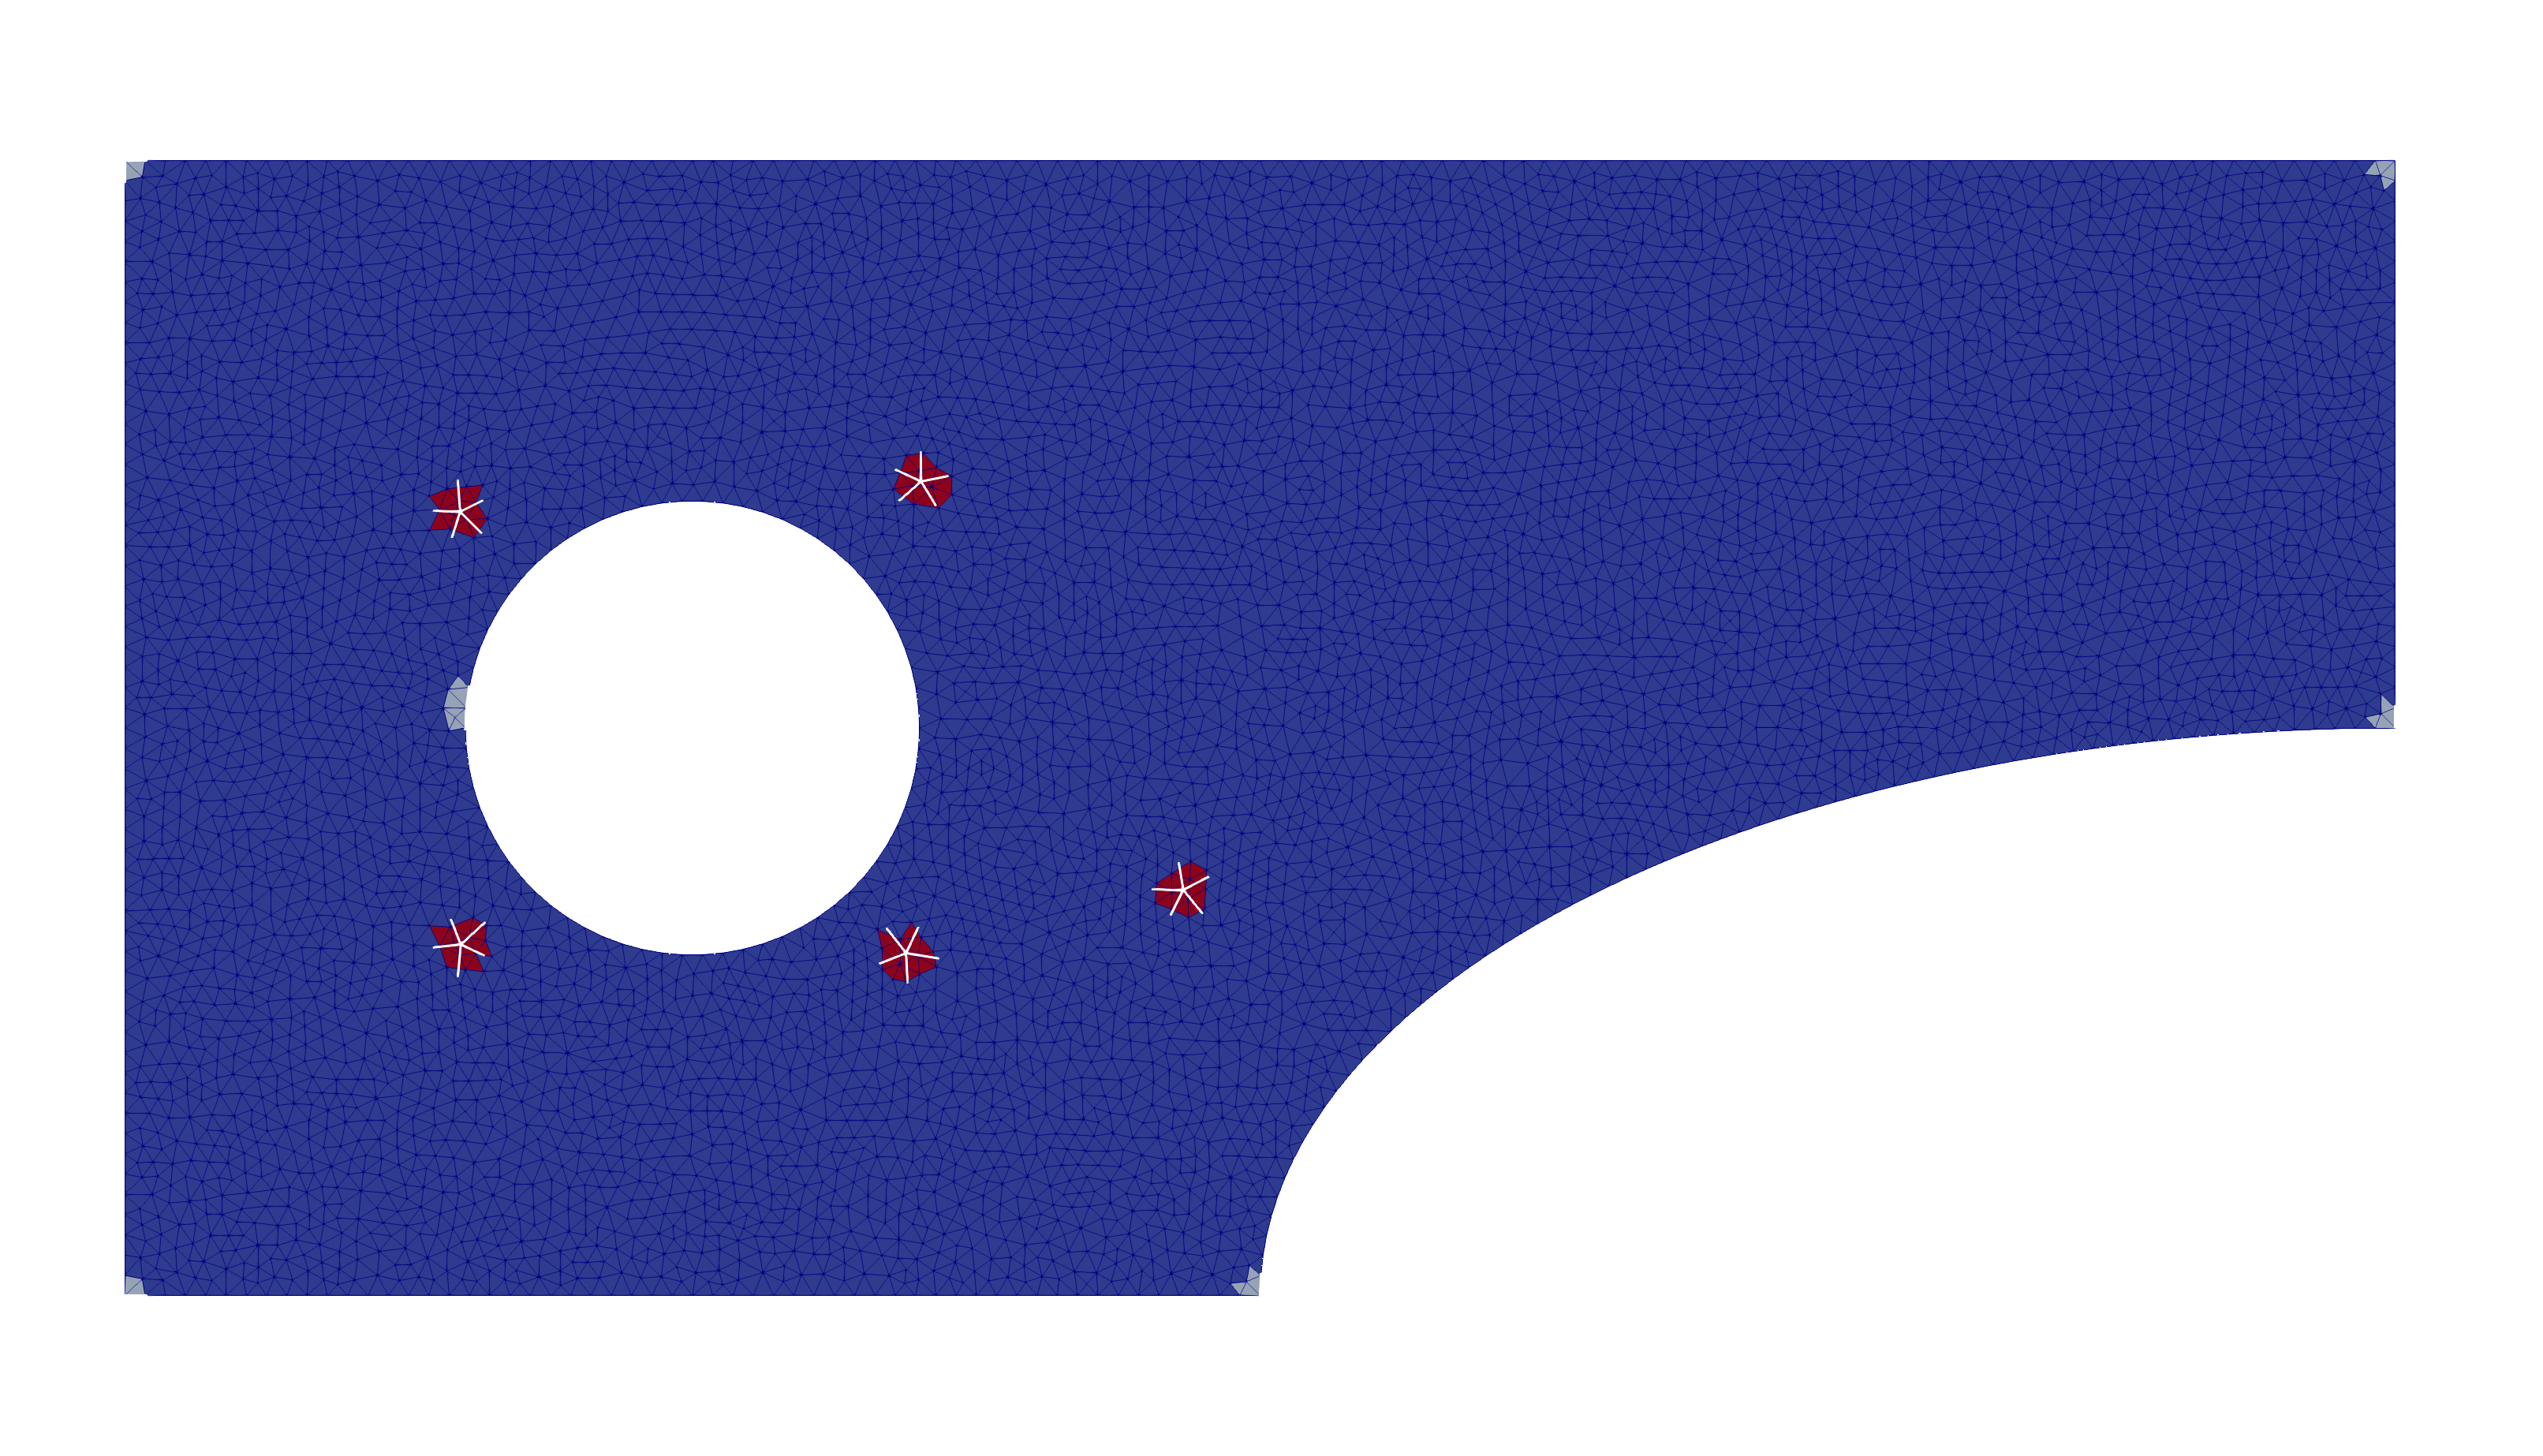
\includegraphics[height=3.7cm]{sing_slots}
%\end{center}
%\captionof{figure}{dfdgd}

%\begin{itemize}

%	\item \textbf{Proposed Solutions}

%	\item Tbbbr

%\end{itemize}
%\smallskip
%}


%----------------------------------------------------------------------------------------
%	Expected contribution and Impact
%----------------------------------------------------------------------------------------
%%%%%%%%%%%%%%%%%%%%%%%%%%%%%%%%%%%%%%%%%%%%%%%%%%%%%%%%%%%%%%%%%%%%%
%\headerbox{Conclusions and Perspectives}{name=conclusion,column=1,below=experimentation}{
%%%%%%%%%%%%%%%%%%%%%%%%%%%%%%%%%%%%%%%%%%%%%%%%%%%%%%%%%%%%%%%%%%%%%
%\medskip
%
%\smallskip
%\begin{itemize}
%\item Continuous strategies 
%\newline
% - better CF approximation (used methods: Heun or RK4)
% \newline
% - depend on proximity parameter and does not always find a valid result
% \newline
% - influence of mesh resolution - not obvious
% \newline
%\item Discrete strategy
%\newline 
%- guaranteed to find a result (importance of final choice)
%\newline
%- depends only on mesh resolution (straightforward influence: higher resolution $\rightarrow$ better approximation) 
%\item The discrete strategy is applied to the triangles of the mesh; it can be further refined by making use of the vertices as well.
%\item post-process for discrete strategy: refine detected streamlines using a continuous approach 
%\end{itemize}
%\smallskip
%}

\headerbox{Conclusions and Perspectives}{name=conclusion,column=0,row=0,span=2,above=bottom}{

\noindent
\begin{minipage}[b]{0.49\linewidth}
\begin{tcolorbox}[colframe=gray,boxrule=0.1pt,title=\Large Conclusions]	
\begin{itemize}
\item Continuous strategies 
\newline
 - better CF approximation (used methods: Heun or RK4)
 \newline
 - depend on proximity parameters and do not always find a valid result
 \newline
 - influence of mesh resolution - not obvious
\item Discrete strategy
\newline 
- guaranteed to find a result (importance of final choice)
\newline
- depends only on the mesh resolution (straightforward influence: higher resolution $\rightarrow$ better approximation) 
\end{itemize}
\end{tcolorbox}
\end{minipage}
\hspace{0.005\linewidth}
\begin{minipage}[b]{0.49\linewidth}
\begin{tcolorbox}[colframe=gray,boxrule=0.1pt,title=\Large Perspectives - Discrete Strategy]	
\begin{itemize}
\item We obtain all possible solutions for the singularity lines between singularity slots, however we do not have a final Singularity Graph; a strategy such as the Minimum Spanning Tree can be applied. 
\item The strategy is applied to a graph with the nodes as the original triangle centers; it can be further refined by encompassing the vertices as well.
\item Post-process procedure: refine the detected streamlines using a continuous approach. 
\end{itemize}
\end{tcolorbox}
\end{minipage}
}



%----------------------------------------------------------------------------------------
%	References
%----------------------------------------------------------------------------------------
%%%%%%%%%%%%%%%%%%%%%%%%%%%%%%%%%%%%%%%%%%%%%%%%%%%%%%%%%%%%%%%%%%%%%
%\headerbox{References}{name=refs,column=1,below=results,above=bottom}{
%%%%%%%%%%%%%%%%%%%%%%%%%%%%%%%%%%%%%%%%%%%%%%%%%%%%%%%%%%%%%%%%%%%%%
%\renewcommand{\section}[2]{\vskip 0.05em} % Get rid of the default "References" section title
%\bibliographystyle{unsrt}
%\bibliography{biblio_hpcs} % Use sample.bib as the bibliography file
%}
%----------------------------------------------------------------------------------------

\end{poster}

\end{document}
